\documentclass{bmstu}

\bibliography{biblio}

\begin{document}


\makecourseworktitle
    {Информатика, искусственный интеллект и системы управления} % Название факультета
    {Программное обеспечение ЭВМ и информационные технологии} % Название кафедры
    {Разработка приложения для хранения и анализа информации о киберспортивных матчах и командах} % Тема работы
    {ИУ7-66Б} % Номер группы
    {Леонов~В.~В.} % ФИО студента
    {Кивва~К.~А.} % ФИО научного руководителя
    {}
    {}
    
\setcounter{page}{3}
\begin{essay}{}
    \noindent\textbf{Ключевые слова}: Базы Данных, PostgreSQL, Golang, реляционная модель данных, киберспорт, Dota 2.\\
    
    Целью курсовой работы является проектирование и реализация базы данных, содержащей информацию о киберспортивных матчах и командах в дисциплине Dota 2.
  
	Для достижения указанной цели были выполнены следующие задачи:
	\begin{itemize}
		\item рассмотреть существующие сервисы;
		\item формализовать задание и определить необходимый функционал;
  	\item спроектировать базу данных, описать ее сущности и связи;
		\item выбрать подходящую систему управления базами данных;
        \item реализовать базу данных;
        \item провести сравнительный анализ времени обработки запроса в базе данных с индексацией и без;
		\item реализовать программное обеспечение, которое позволит получить доступ к данным.
	\end{itemize}
    
   Цель курсовой работы была достигнута в полном объеме: была изучена предметная область, были выполнены проектирование и реализация базы данных, содержащей информацию о киберспортивных матчах и командах в дисциплине Dota 2, были созданы соответствующие триггеры и проведено исследование влияния индексации записей на скорость выполнения запросов в базе данных.
\end{essay}

\maketableofcontents

\chapter*{ВВЕДЕНИЕ}
\addcontentsline{toc}{chapter}{ВВЕДЕНИЕ}

Сегодня, в век высоких технологий, наравне с общеизвестными спортивными дисциплинами звучит слово <<киберспорт>> и привлекает интерес большого количества людей. Как и в любом виде спорта в киберспорте проводится множество турниров различного уровня во всех регионах с обширным количеством игроков, спонсоров и матчей внутри конкретного соревнования. Одной из самых популярных дисциплин и с огромным количеством зрителей является Dota 2 \cite{twitchtracker}.

Многие люди имеют любимые команды, фаворитов среди игроков и следят за их карьерой. Таким образом, существует потребность в сервисе, предоставляющем данные о турнирах, командах, внутриматчевую или глобальную статистику выступлений и другую сопутствующую информацию.

Целью курсовой работы является проектирование и реализация базы данных, содержащей информацию о киберспортивных матчах и командах в дисциплине Dota 2.

Для достижения указанной выше цели следует выполнить следующие задачи:
	\begin{itemize}
		\item рассмотреть существующие сервисы;
		\item формализовать задание и определить необходимый функционал;
  	\item спроектировать базу данных, описать ее сущности и связи;
		\item выбрать подходящую систему управления базами данных;
        \item реализовать базу данных;
        \item провести сравнительный анализ времени обработки запроса в базе данных с индексацией и без;
		\item реализовать программное обеспечение, которое позволит получить доступ к данным.
	\end{itemize}

\chapter{Аналитический раздел}

В аналитическом разделе выполнено изучение предметной области, представлено формальное описание данных, выполнен анализ существующих моделей и методов организации хранения данных в базе знаний.

\section{Постановка задачи}

Необходимо спроектировать и реализовать базу данных, содержащую информацию о киберспортивных матчах и командах в дисциплине Dota 2. Следует разработать интерфейс, который позволит работать с этой базой данных: добавлять, удалять и редактировать информацию, составлять отчеты по периодам, задаваемым пользователем, с их графическим представлением. Требуется предусмотреть наличие ролей модератора и администратора, осуществляющих контроль за добавлением новых турниров, регистрацией новых команд и обновлением текущих составов.

\section{Актуальность проекта}

С каждым годом призовые фонды турниров становятся все больше. Более того, киберспортивные первенства проходят даже в пределах конкретных организаций, школ, колледжей, университетов и других объединений, которые в свою очередь нельзя подробно изучить в одном месте.

Российская команда Team Spirit стала победителем The International 10, что существенным образом сказалось на популярности и интересе к киберспортивной составляющей Dota 2 \cite{teamspirit}.

Таким образом, разрабатываемое приложение предложит удобный инструмент для просмотра статистики по киберспортивным турнирам, с возможностями добавления своих и составления отчетов за выбранный период.

\section{Предметная область}

\subsection{Краткое описание игрового процесса}

Dota 2 представляет собой соревновательную командную игру с RPG (англ. Role-Playing Game --- ролевая игра) элементами типа MOBA (<<многопользовательская онлайновая боевая арена>>). Две соревнующиеся команды Света (англ. The Radiant) и Тьмы (англ. The Dire) состоят из пяти игроков каждая. Главной целью игры в Dota 2 является уничтожение вражеской крепости (англ. Ancient). Каждая из крепостей защищается несколькими башнями, расположенными вдоль трех линий обороны. Вместо построения собственной армии как в классических RTS играх (англ. Real Time Strategy --- Стратегии реального времени), каждый игрок управляет одним уникальным героем с отличительными умениями, узнаваемой внешностью, силами, слабостями и уникальным стилем игры \cite{dota2}.


Каждый из игроков выполняет определенную роль на протяжении матча,  как например <<керри>> (англ. Carry) или <<саппорт>> (англ. Support), и герои могут по своим характеристикам лучше подходить для той или иной роли. Во время игры герой имеет возможность зарабатывать опыт и золото, которое можно тратить на покупку предметов, которые позволяют усилить одну или несколько характеристик персонажа: урон по другим героям, восстановление здоровья или потенциал уничтожения вражеских строений. 

Если очки здоровья героя снижаются до нуля — например, его одолевает в бою вражеский герой --- герой в течение некоторого короткого времени считается <<погибшим>>; по окончании этого времени герой вновь появляется рядом с крепостью, и управляющий им игрок может возобновить игру. Убийство врага позволяет получить большое количество дополнительного золота и опыта.

\subsection{Dota Pro Circuit}

Dota Pro Circuit --- профессиональные турниры организуются компанией Valve и её партнёрами, для определения команд, которые получат прямые приглашения на The International (главный турнир года).

Заработанные за сезон баллы будут определять статус команды перед The International и её шансы на получение прямого приглашения \cite{dpc}.

\section{Обзор существующих сервисов}

Следует отметить, что существуют сервисы, которые агрегируют, систематизируют и визуализируют информацию о киберспортивных турнирах.

DOTABUFF является крупнейшим сервисом для сбора и анализа матчевой статистики, в том числе о профессиональных матчах. Однако, данный сервис доступен только на английском языке и помимо киберспортивной информации имеет множество дополнительной, которая несколько осложняет взаимодействие (см. рисунок \ref{fig:dotabuff}).

\begin{figure}[h!btp]
	\centering
	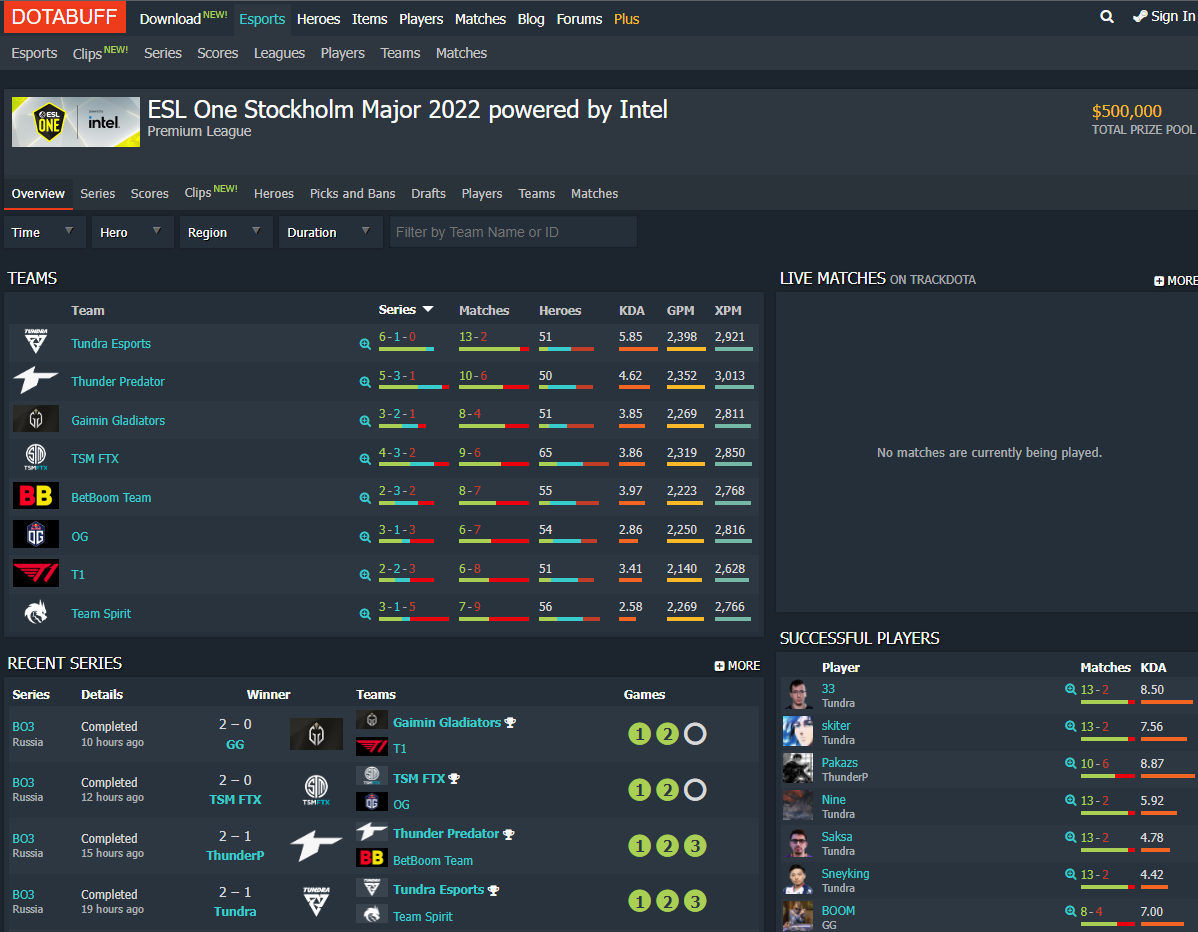
\includegraphics[width=450pt]{inc/img/dotabuff.png}
	\caption{Портал dotabuff.com}
	\label{fig:dotabuff}	
\end{figure}

OpenDota --- это проект энтузиастов с открытым исходным кодом, собирающий данные Dota 2. Сервис предоставляет веб-интерфейс для обычных пользователей, так же как API для разработчиков с возможностью интеграции в сторонние приложения. Большим плюсом является возможность детального изучения матча с автоматизированной аналитикой и советами  (см. рисунок \ref{fig:opendota}) \cite{opendota}.

\begin{figure}[h!btp]
	\centering
	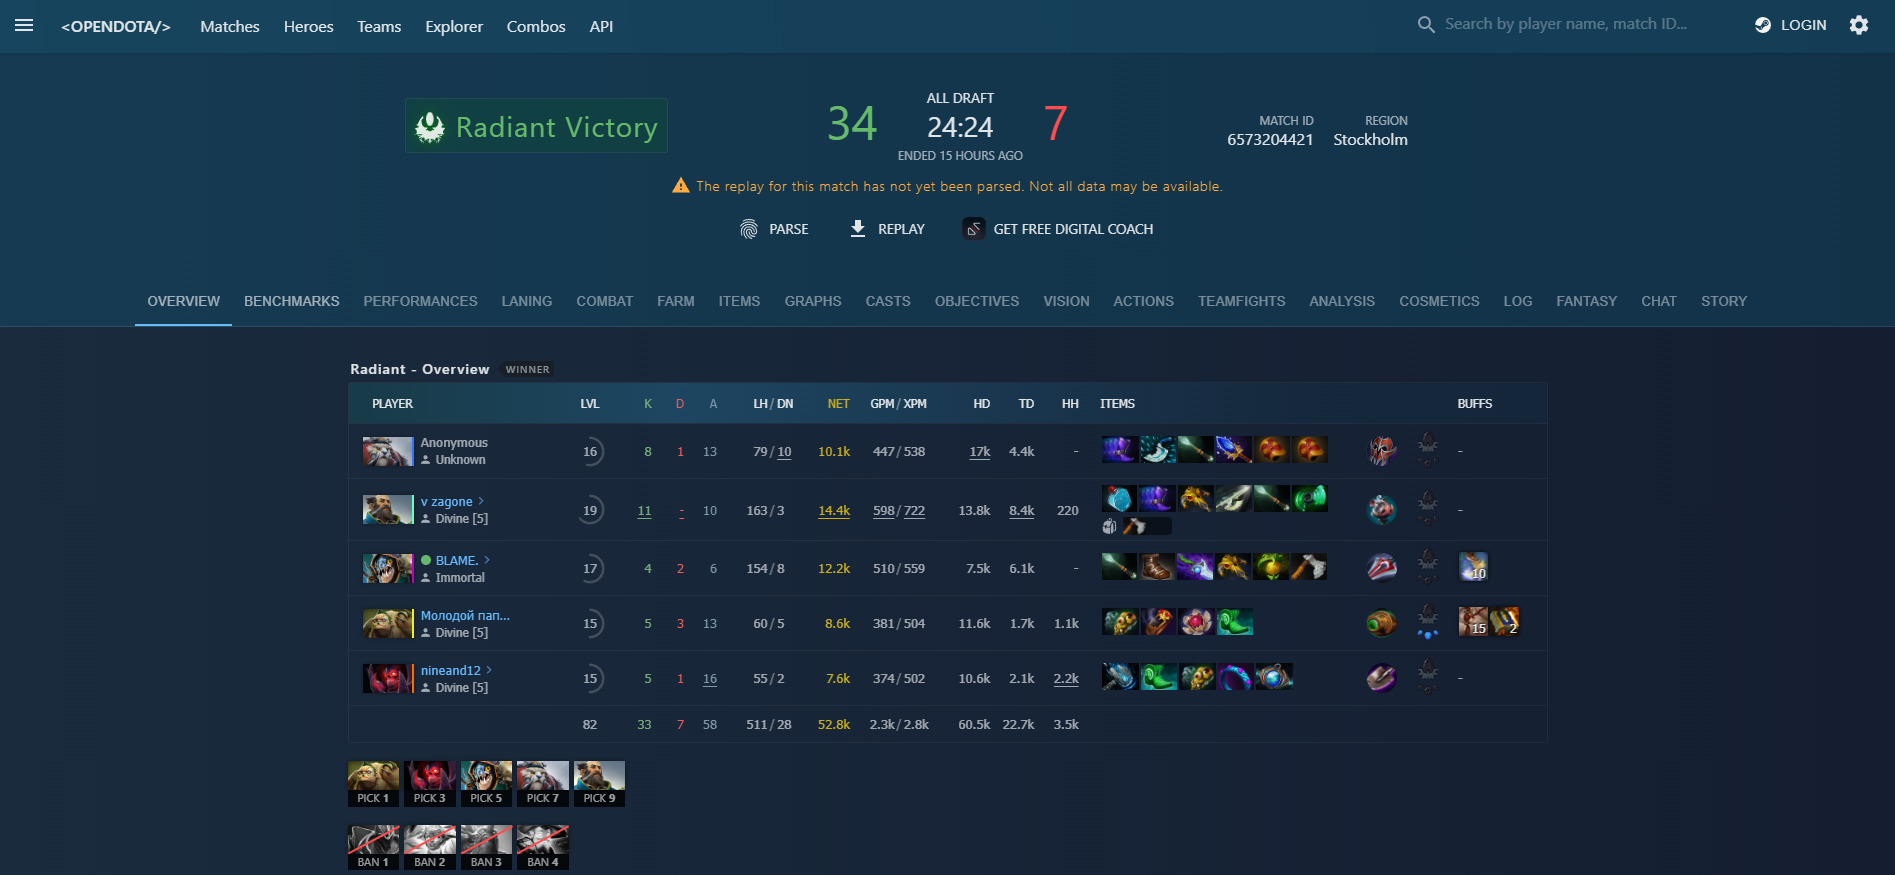
\includegraphics[width=450pt]{inc/img/opendota.png}
	\caption{Портал opendota.com}
	\label{fig:opendota}	
\end{figure}

\newpage

На рисунке \ref{fig:cybersport} представлен портал cybersport.ru. Данный сервис специализируется на широком круге киберспортивных дисциплин. Портал позволяет смотреть матчи в прямом эфире, следить за турнирной сеткой, читать новости о профессиональных игроках и командах, но не дает пользователю подробной статистики и послематчевой аналитики. Доступность на русском языке выгодно выделяет сервис на фоне конкурентов.

\begin{figure}[h!btp]
	\centering
	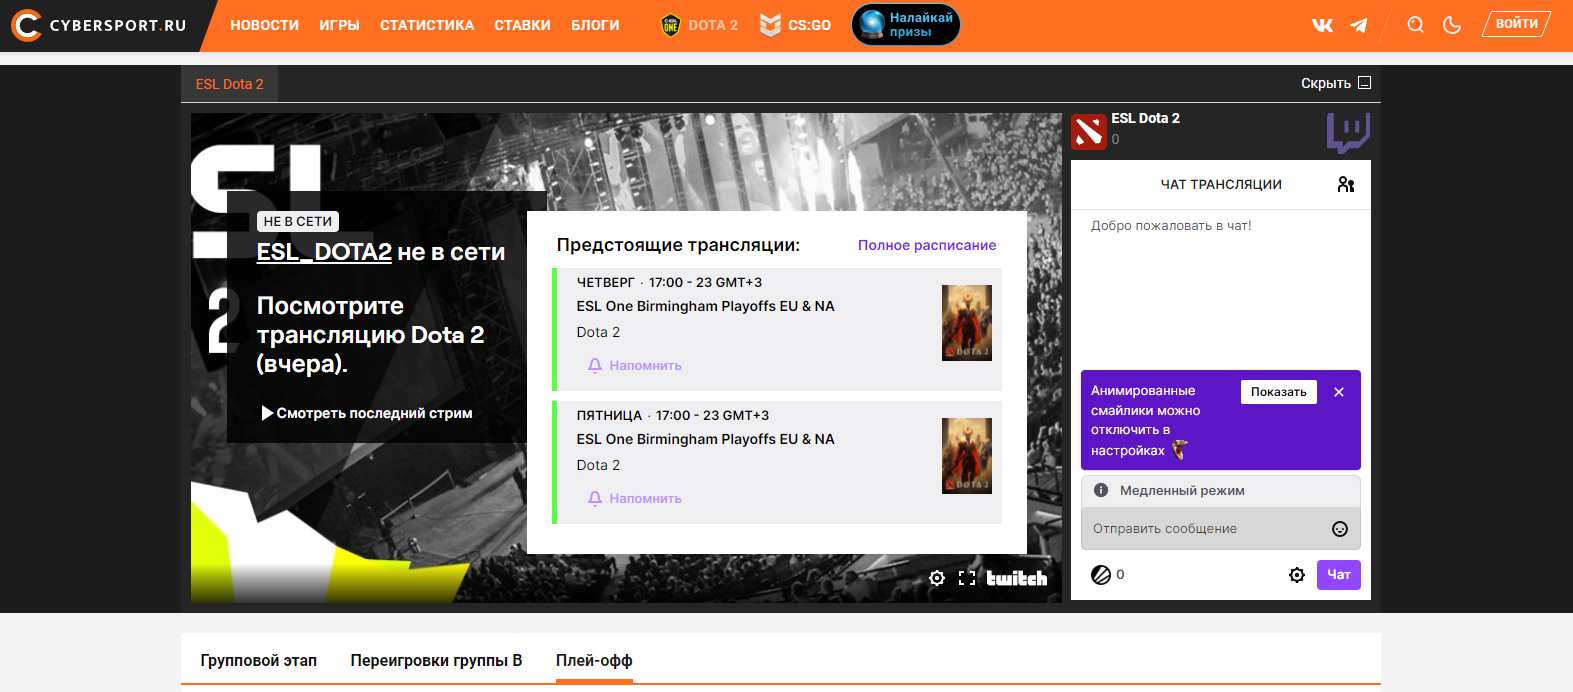
\includegraphics[width=450pt]{inc/img/cybersport.png}
	\caption{Портал cybersport.ru}
	\label{fig:cybersport}	
\end{figure}

Таким образом, на основе рассмотренных сервисов можно составить сравнительную таблицу \ref{tabular:services}.

\begin{table}[h!]
	\centering
	\caption{\label{tabular:services}Сравнительная таблица сервисов}
	\begin{tabular}{|p {5 cm}|p {3cm}|p {3cm}|p {3.5 cm}|}
		\hline
		\textbf{} & \textbf{DOTABUFF} & \textbf{OpenDota} & \textbf{cybersport.ru} \\ \hline
		\textbf{Открытый исходный код} & - & + & - \\ \hline
		\textbf{Доступность} & По подписке & Бесплатно & С рекламой \\ \hline
		\textbf{Послематчевая статистика} & + & + & - \\ \hline
		\textbf{Турниры} & - & - & + \\ \hline
		\textbf{Язык} & Английский & Английский & Русский \\ \hline
		\textbf{Наличие desktop-приложения} & + & - & - \\ \hline
	\end{tabular}
	
\end{table}

Ни один из представленных сервисов не обладает desktop-приложением, возможностью просмотра турниров и доступностью на русском языке. Разрабатываемое ПО должно соответствовать этим требованиям.

\newpage

\section{Типы пользователей}

Разрабатываемая система ориентирована на многопользовательское использование, следовательно, важным является разделение пользователей по ролям и соответствующему им функционалу (таблица \ref{tabular:users_info}).

\begin{table}[h!]
	\centering
	\caption{\label{tabular:users_info}Типы пользователей и доступный им функционал}
	\begin{tabular}{|p{5 cm}|p{10 cm}|}
		\cline{1-2}
		\textbf{Тип пользователя}  & \textbf{Доступный функционал}                                                                           \\ \cline{1-2}
		Неавторизованный & Регистрация, авторизация \\ \cline{1-2}
		Клиент & Просмотр информации о киберспортивных матчах, прошедших турнирах, составах команд, сведений о игроках и сводной статистики за заданный период\\ \cline{1-2}
		Модератор & Просмотр информации о киберспортивных матчах, прошедших турнирах, составах команд, сведений о игроках и сводной статистики за заданный период
		\newline
		Операции доступа, изменения и удаления информации в базе знаний \\ \cline{1-2}
		Администратор & Просмотр информации о киберспортивных матчах, прошедших турнирах, составах команд, сведений о игроках и сводной статистики за заданный период
		\newline
		Операции доступа, изменения и удаления информации в базе знаний
		\newline 
		Добавление и удаление пользователей, изменение типа существующего пользователя \\ \cline{1-2}
	\end{tabular}%
\end{table}

Возможные варианты взаимодействия с системой описаны при помощи UseCase--диаграммы, которая приведена на рисунке \ref{fig:use_case}.

\begin{figure}[h!btp]
	\centering	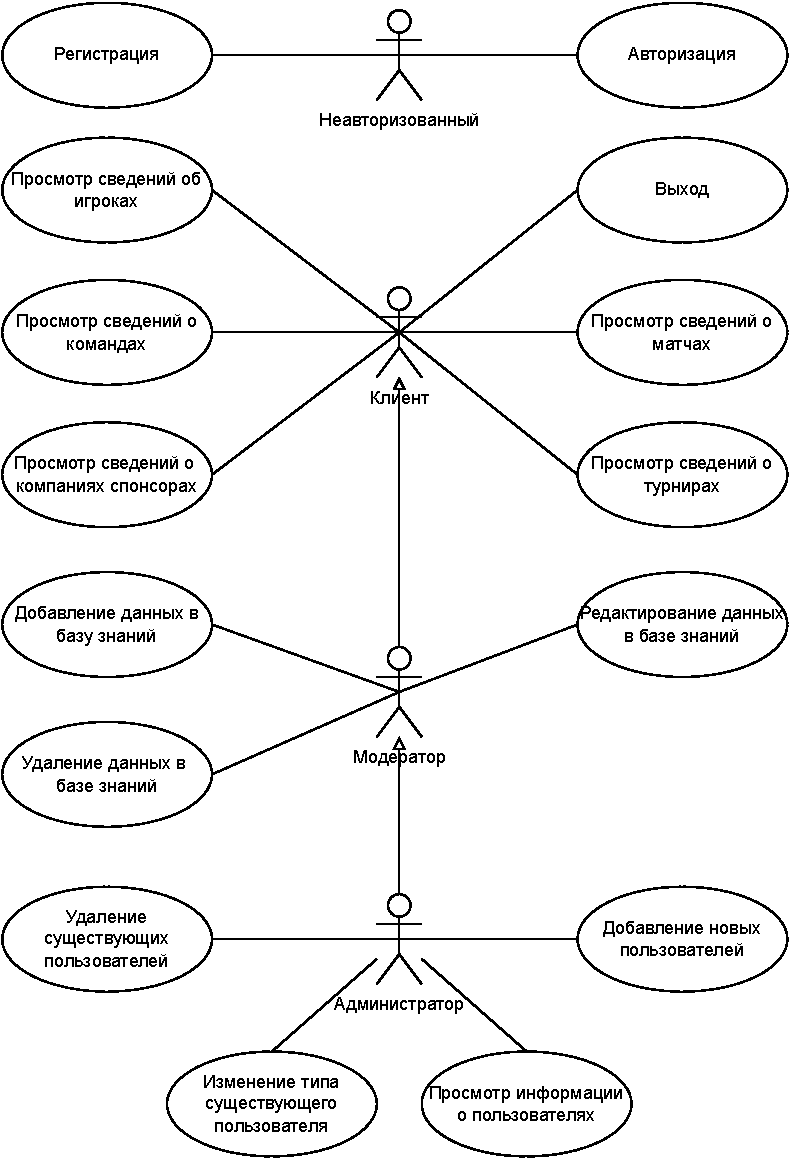
\includegraphics[width=450pt]{inc/diag/use_case.pdf}
	\caption{UseCase-диаграмма}
	\label{fig:use_case}	
\end{figure}

\newpage

\section{Формализация данных}

База данных должна хранить информацию о: 
\begin{itemize}
	\item турнирах;
	\item компаниях-спонсорах;
	\item командах;
	\item игроках;
	\item матчах;
	\item пользователях.
\end{itemize}

В таблице \ref{tabular:data_info} описано формальное представление данных и сведения, которые они содержат.

\begin{table}[h!]
	\centering
	\caption{\label{tabular:data_info}Данные и сведения о них}
	\begin{tabular}{|p{3 cm}|p{12 cm}|}
		\cline{1-2}
		\textbf{Данные}  & \textbf{Сведения}                                                                           \\ \cline{1-2}
		Турнир           & Название, уровень, призовой фонд, дата, время и место проведения, количество DPC очков   \\ \cline{1-2}
		Компания-спонсор & Название, страна, вебсайт, ежегодная выручка, область деятельности                \\ \cline{1-2}
		Команда          & Название, дата создания, контактный e-mail, общий заработок, регион, уровень             \\ \cline{1-2}
		Игрок            & Псевдоним, имя, дата рождения, страна, личный рейтинг, игровая позиция, сигнатурный герой   \\ \cline{1-2}
		Матч             & Продолжительность, победитель, герои, соотношение убийств, смертей и помощи, общая ценность, опыт и золото в минуту, урон\\ \cline{1-2}
		Пользователь     & Логин, пароль, права доступа, e-mail, имя                                                 \\ \cline{1-2}
	\end{tabular}%
\end{table}

На основе выделенных данных и сведений, которые они содержат, следует составить диаграмму в нотации Чена, описывающую сущности исследуемой системы, а также их взаимодействие (рисунок \ref{fig:chen}).

\newpage

\begin{figure}[h!btp]
	\centering
	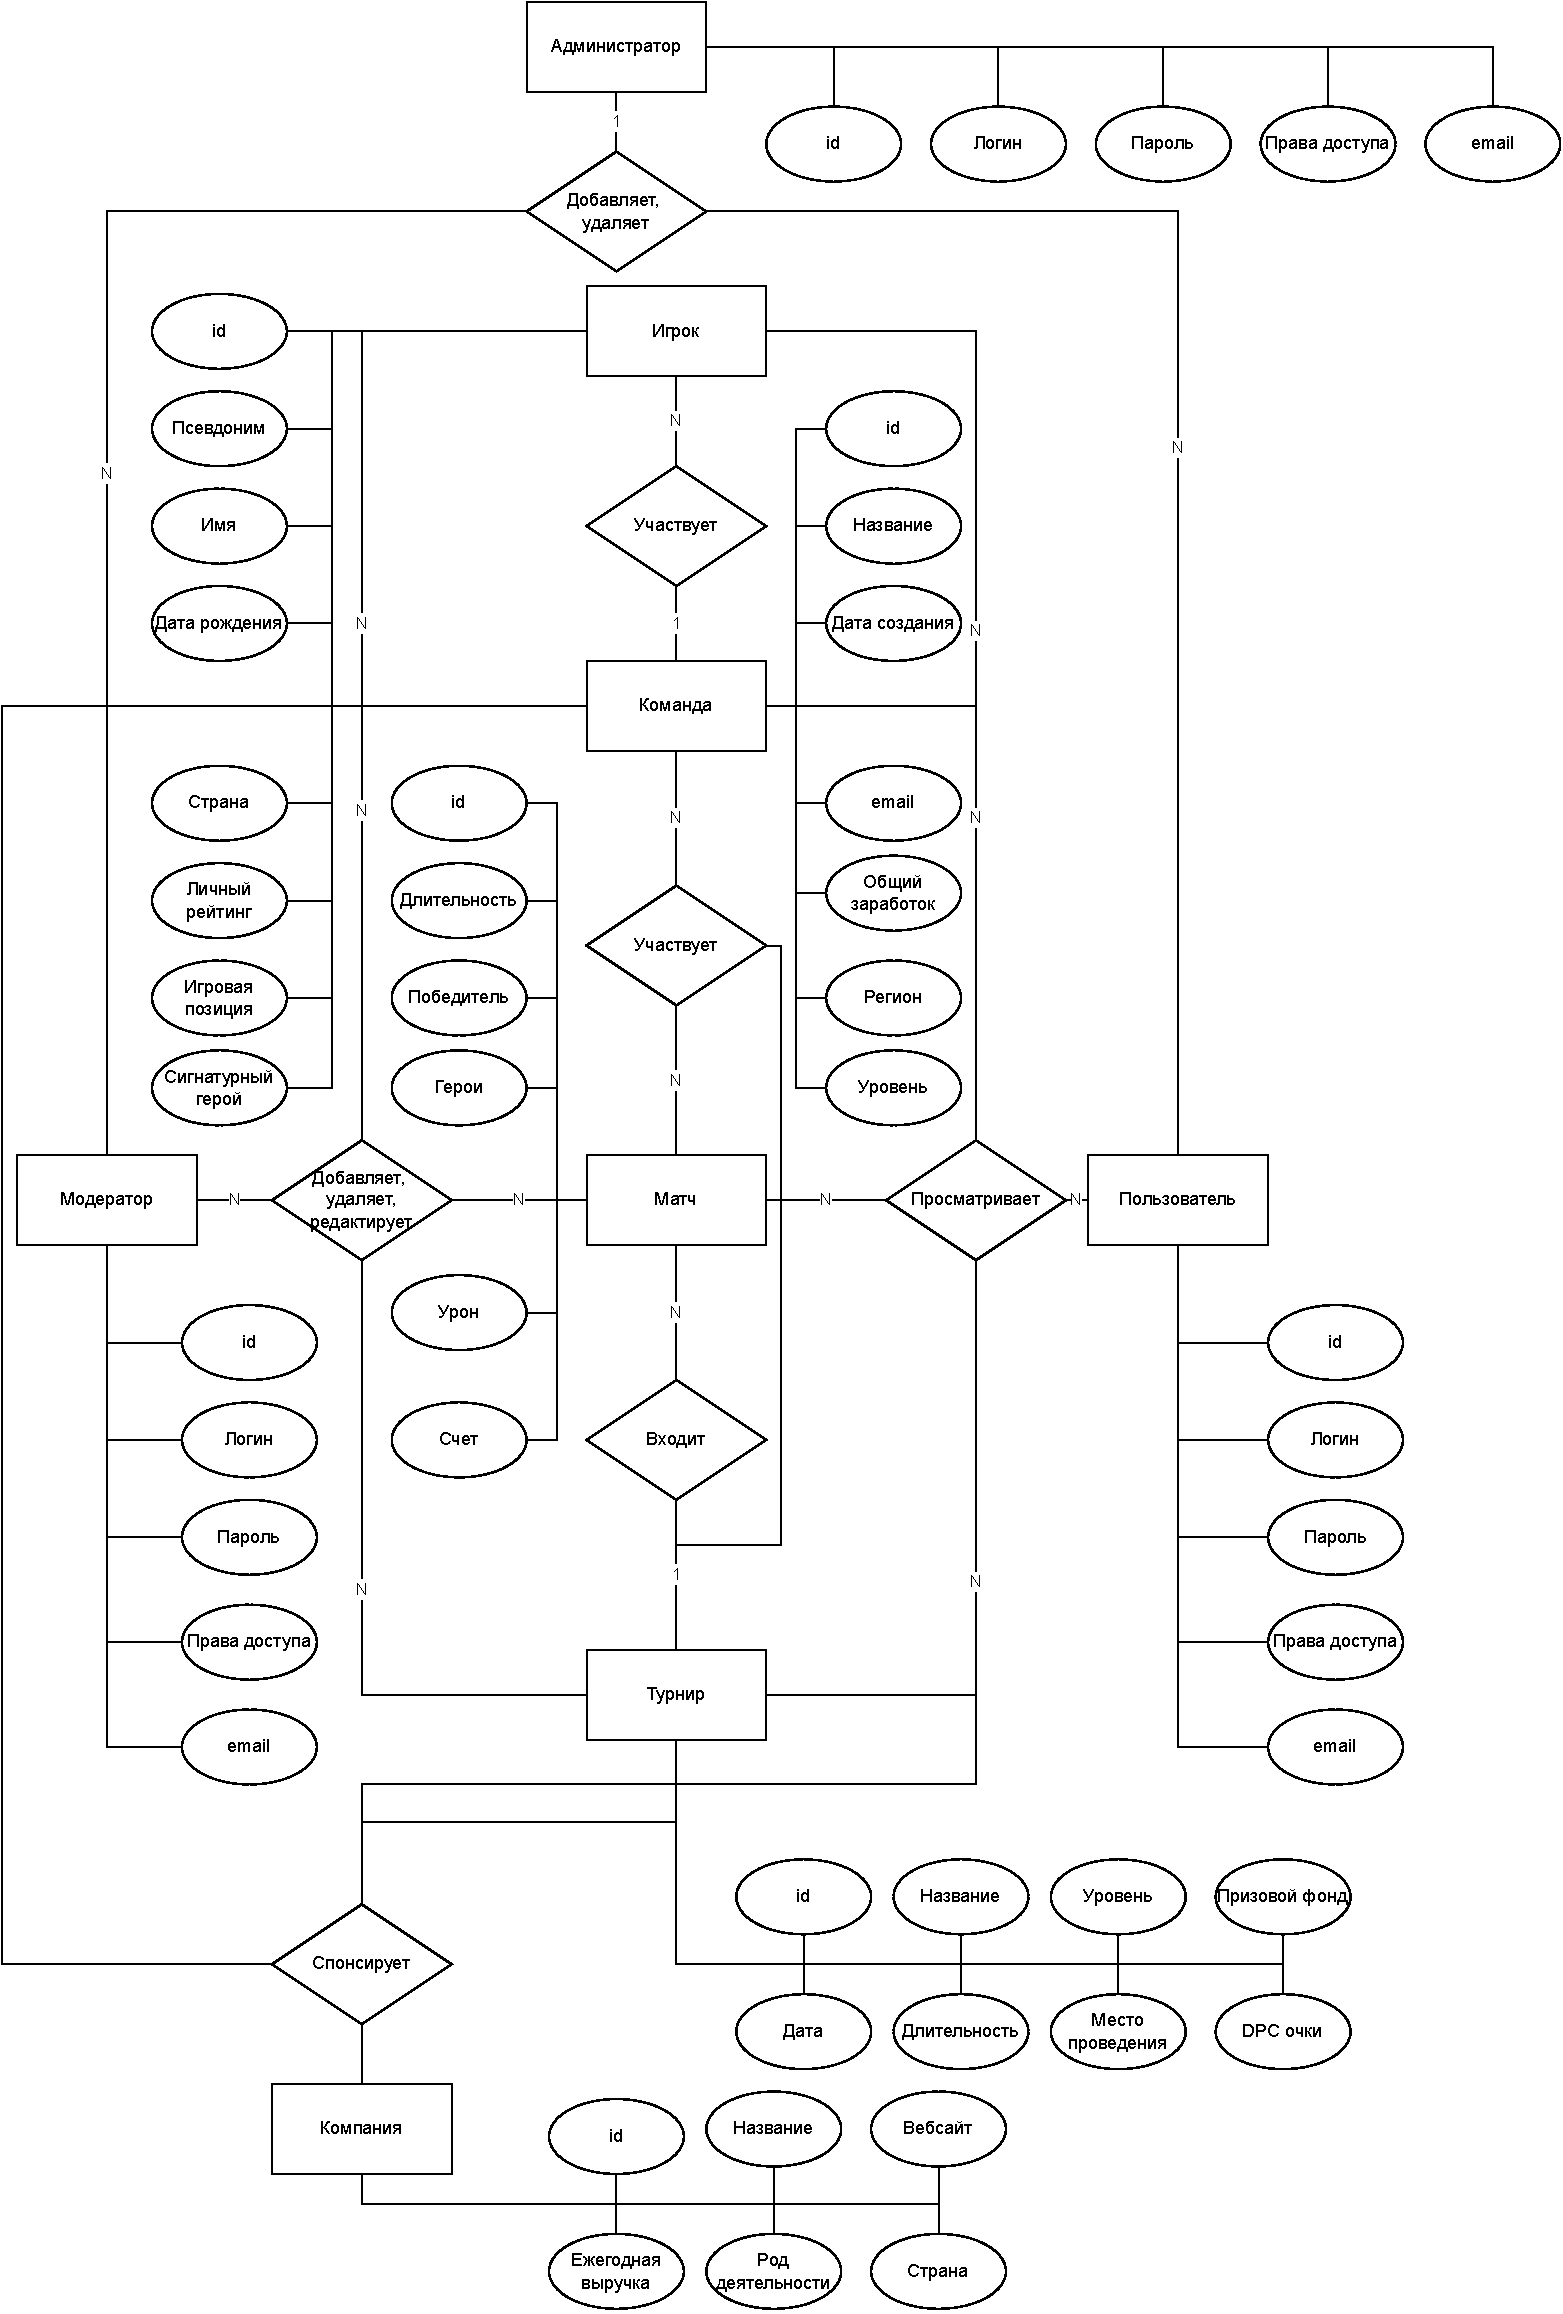
\includegraphics[width=450pt]{inc/diag/chen.pdf}
	\caption{Диаграмма сущность--связь}
	\label{fig:chen}	
\end{figure}

\newpage


\section{Выводы}

В данном разделе было выполнено изучение предметной области, представлено формальное описание данных, возможные варианты взаимодействия с системой описаны при помощи UseCase--диаграммы, а также составлена диаграмма сущность--связь предметной области. 



\chapter{Конструкторский раздел}
\section{Схемы базы данных}

База данных должна включать следующие таблицы: 
\begin{itemize}
	\item таблица о турнирах --- \code{Tournaments};
	\item таблица о компаниях-спонсорах --- \code{Companies};
	\item таблица о командах --- \code{Teams};
	\item таблица о игроках --- \code{Players};
	\item таблица о матчах --- \code{Matches};
	\item таблица о пользователях --- \code{Users}.
\end{itemize}

Далее представлено подробное описание полей, каждой из таблиц. Диаграмма базы данных изображена на рисунке \ref{fig:database}.

Таблица \code{Tournaments} описывает турниры и содержит следующие поля:
\begin{itemize}
	\item \code{id} --- идентификатор турнира (первичный ключ), представляется целым числом;
	\item \code{name} --- название турнира, представляется строкой;
	\item \code{tier} --- уровень престижности турнира, представляется целым числом;
	\item \code{prize\_pool} --- призовой фонд турнира, представляется целом числом;
	\item \code{data\_start} --- дата начала проведения турнира, представляется типом дата;
	\item \code{duration} --- продолжительность турнира в днях, представляется целым числом;
	\item \code{dpc\_points} --- количество DPC-очков на турнире, представляется целым числом;
	\item \code{location} --- место проведения турнира, представляется строкой.
\end{itemize}
\clearpage

\begin{figure}[h!btp]
	\centering \includegraphics[width=\textwidth, page=2]{inc/img/database.png}
	\caption{Диаграмма базы данных}
	\label{fig:database}	
\end{figure}

Таблица \code{Companies} описывает компании-спонсоры и содержит следующие поля:
\begin{itemize}
	\item \code{id} --- идентификатор компании (первичный ключ), представляется целым числом;
	\item \code{name} --- название компании, представляется строкой;
	\item \code{country} --- страна компании, представляется строкой;
	\item \code{website} --- вебсайт компании, представляется строкой;
	\item \code{revenue} --- годовой оборот компании, представляется целым типом;
	\item \code{industry} --- сфера деятельности компании. 
\end{itemize}

\newpage

Таблица \code{Teams} описывает команды и содержит следующие поля:
\begin{itemize}
	\item \code{id} --- идентификатор команды (первичный ключ), представляется целым числом;
	\item \code{name} --- название команды, представляется строкой;
	\item \code{created\_at} --- дата создания команды, представляется типом дата;
	\item \code{email} --- email команды, представляется строкой;
	\item \code{total\_earnings} --- общий заработок команды, представляется целым типом;
	\item \code{region} --- регион, который представляет команда, представляется строкой;
	\item \code{tier} --- уровень команды, представляется целым типом. 
\end{itemize}

Таблица \code{Players} описывает игроков и содержит следующие поля:
\begin{itemize}
	\item \code{id} --- идентификатор игрока (первичный ключ), представляется целым числом;
	\item \code{nickname} --- псевдоним игрока, представляется строкой;
	\item \code{realname} --- имя игрока, представляется строкой;
	\item \code{birthdate} --- дата рождения игрока, представляется типом дата;
	\item \code{country} --- страна игрока, представляется строкой;
	\item \code{mmr} --- личный рейтинг игрока, представляется целым числом;
	\item \code{role} --- избранная роль игрока, представляется строкой;
	\item \code{signature\_hero} --- избранный герой игрока, представляется строкой.
\end{itemize}

Таблица \code{Matches} описывает матчи и содержит следующие поля:
\begin{itemize}
	\item \code{id} --- идентификатор матча (первичный ключ), представляется целым числом;
	\item \code{tournament\_id} --- идентификатор турнира (является ссылкой на таблицу \code{Tournaments}), представляется целым числом;
	\item \code{r\_team\_id} --- идентификатор команды Света (является ссылкой на таблицу \code{Teams}), представляется целым числом;
	\item \code{d\_team\_id} --- идентификатор команды Тьмы (является ссылкой на таблицу \code{Teams}), представляется целым числом;
	\item \code{duration} --- продолжительность матча, представляется целым числом;
	\item \code{winner} --- победитель матча, представляется логическим типом.
\end{itemize}

Таблица \code{Users} описывает пользователей и содержит следующие поля:
\begin{itemize}
	\item \code{id} --- идентификатор пользователя (первичный ключ), представляется целым числом;
	\item \code{name} --- имя пользователя, представляется строкой;
	\item \code{birthdate} --- дата рождения пользователя, представляется типом дата;
	\item \code{login} --- логин пользователя, представляется строкой;
	\item \code{password} --- пароль пользователя, представляется строкой;
	\item \code{email} --- email пользователя, представляется строкой;
	\item \code{privilege\_level} --- уровень привилегий пользователя, представляется целым числом.
\end{itemize}

Таблицы \code{Tournaments}-\code{Teams} образуют связь многие-ко-многим. Необходимо создать развязочную таблицу \code{Tournaments\_Teams}, которая будет содержать следующие поля:
\begin{itemize}
	\item \code{id} --- идентификатор записи (первичный ключ), представляется целым числом;
	\item \code{tournament\_id} --- идентификатор турнира (является ссылкой на таблицу \code{Tournaments}), представляется целым числом;
	\item \code{team\_id} --- идентификатор команды (является ссылкой на таблицу \code{Teams}), представляется целым числом;
	\item \code{participation\_type} --- способ отбора на турнир, представляется строкой;
	\item \code{is\_winner} --- является ли команда победителем, представляется логическим типом.
\end{itemize}

Таблицы \code{Сompanies}-\code{Tournaments} образуют связь многие-ко-многим. Необходимо создать развязочную таблицу \code{Companies\_Tournaments}, которая будет содержать следующие поля:
\begin{itemize}
	\item \code{id} --- идентификатор записи (первичный ключ), представляется целым числом;
	\item \code{company\_id} --- идентификатор компании (является ссылкой на таблицу \code{Companies}), представляется целым числом;
	\item \code{tournament\_id} --- идентификатор турнира (является ссылкой на таблицу \code{Tournaments}), представляется целым числом;
	\item \code{deposit} --- величина инвестиции компании, представляется целым числом.
\end{itemize}

Таблицы \code{Сompanies}-\code{Teams} образуют связь многие-ко-многим. Необходимо создать развязочную таблицу \code{Companies\_Teams}, которая будет содержать следующие поля:
\begin{itemize}
	\item \code{id} --- идентификатор записи (первичный ключ), представляется целым числом;
	\item \code{company\_id} --- идентификатор компании (является ссылкой на таблицу \code{Companies}), представляется целым числом;
	\item \code{team\_id} --- идентификатор команды (является ссылкой на таблицу \code{Teams}), представляется целым числом;
	\item \code{contract\_date} --- дата подписания контракта, представляется типом дата;
	\item \code{contract\_time} --- срок контракта в месяцах, представляется целым числом.
\end{itemize}

Таблицы \code{Teams}-\code{Players} образуют связь многие-ко-многим. Необходимо создать развязочную таблицу \code{Teams\_Players}, которая будет содержать следующие поля:
\begin{itemize}
	\item \code{id} --- идентификатор записи (первичный ключ), представляется целым числом;
	\item \code{team\_id} --- идентификатор команды (является ссылкой на таблицу \code{Teams}), представляется целым числом;
	\item \code{player\_id} --- идентификатор игрока (является ссылкой на таблицу \code{Players}), представляется целым числом;
	\item \code{contract\_date} --- дата подписания контракта, представляется типом дата;
	\item \code{contract\_time} --- срок контракта в месяцах, представляется целым числом.
\end{itemize}

\newpage	

Таблицы \code{Matches}-\code{Players} образуют связь многие-ко-многим. Необходимо создать развязочную таблицу \code{Match\_Perfomances}, которая будет содержать следующие поля:
\begin{itemize}
	\item \code{id} --- идентификатор записи (первичный ключ), представляется целым числом;
	\item \code{match\_id} --- идентификатор матча (является ссылкой на таблицу \code{Matches}), представляется целым числом;
	\item \code{player\_id} --- идентификатор игрока (является ссылкой на таблицу \code{Players}), представляется целым числом;
	\item \code{team} --- сторона (Свети или Тьма), представляется логическим типом;
	\item \code{hero} --- герой, представляется строкой;
	\item \code{kills} --- количество убийств, представляется целым числом;
	\item \code{deaths} --- количество смертей, представляется целым числом;
	\item \code{assists} --- количество помощей, представляется целым числом;
	\item \code{networth} --- общая ценность, представляется целым числом;
	\item \code{gpm} --- золото в минуту, представляется целым числом;
	\item \code{xpm} --- опыта в минуту, представляется целым числом;
	\item \code{dmg} --- общий урон по героям, представляется целым числом;
	\item \code{heal} --- общее лечение, представляется целым числом;
	\item \code{bld} --- общий по строениям, представляется целым числом.
\end{itemize}

\newpage

\section{Схемы триггеров}

При заключении нового контракта на спонсорство турнира одной из компании следует увеличивать призовой фонд соответствующего турнира. Для этого используется триггер, схема которого приведена на рисунке \ref{fig:new_sponsorship}.

\begin{figure}[h!btp]
	\centering
	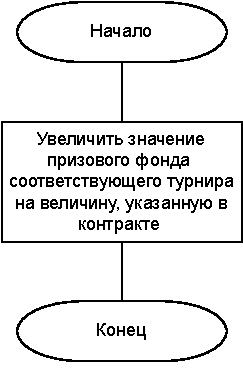
\includegraphics{inc/diag/new_sponsorship.pdf}
	\caption{Схема триггера обновления призового фонда турнира}
	\label{fig:new_sponsorship}	
\end{figure}

При добавлении записи о победе команды в рамках определенного турнира следует увеличивать величину общего заработка команды. Для этого используется триггер, схема которого приведена на рисунке \ref{fig:new_winner}.

\begin{figure}[h!btp]
	\centering
	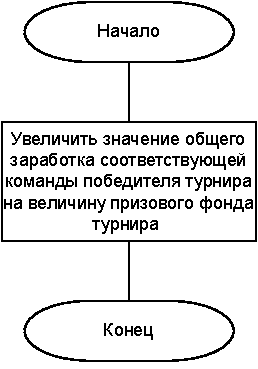
\includegraphics{inc/diag/new_winner.pdf}
	\caption{Схема триггера обновления общего заработка команды}
	\label{fig:new_winner}	
\end{figure}

\section{Выводы}

В данном разделе было выполнено проектирование базы данных, описаны таблицы, которые необходимо реализовать в рамках рассматриваемой задачи, а также разработаны схемы триггеров для базы данных.


\chapter{Технологический раздел}
\label{cha:impl}

Далее в технологическом разделе будут описаны выбранные технологии разработки, методология построения ПО, а также рассмотрено взаимодействие пользователя с приложением.


\section{Выбор технологий разработки}

В качестве СУБД был сделан выбор в пользу PostgreSQL --- это мощная система объектно-реляционных баз данных с открытым исходным кодом, которая использует и расширяет язык SQL в сочетании со многими функциями, позволяющими безопасно хранить и масштабировать самые сложные рабочие нагрузки данных \cite{postgre}.

В качестве ЯП был сделан выбор в пользу Go --- это проект с открытым исходным кодом, призванный повысить продуктивность программистов. Язык Go выразительный, лаконичный, чистый и эффективный. Его механизмы параллелизма упрощают написание программ, максимально использующих многоядерные и сетевые машины, а новая система типов обеспечивает гибкое и модульное построение программ. Go быстро компилируется в машинный код, но обладает удобством сборки мусора и возможностями отражения во время выполнения. Это быстрый, статически типизированный компилируемый язык, который выглядит как динамически типизированный интерпретируемый язык \cite{golang}.

Для разработки программного интерфейса используется Fyne --- это простая в освоении бесплатная платформа с открытым исходным кодом для создания графических приложений для настольных компьютеров, мобильных устройств и других устройств. Сочетая мощь и простоту языка программирования Go с тщательно продуманной библиотекой виджетов разработчику легко создавать приложения и развертывать их \cite{fyne}.

\section{Методология построения ПО}

Разрабатываемое приложение спроектировано на основе чистой архитектуры. Этот способ организации кода подразумевает четкое строгое разделение ответственности. Приложение разбивается на независимые функциональные компоненты, которые взаимодействуют друг с другом определенным образом, при этом между ними передаются только те ресурсы, которые необходимы для выполнения конкретной задачи. Это помогает минимизировать сложность каждого компонента, снизить вероятность ошибок и ускоряет их выявление \cite{cleancode}.

На рисунке \ref{fig:components} представлено высокоуровневое разбиение приложения на компоненты. Данный подход позволяет легко масштабировать приложение, а также выполнять подмену независимых компонентов, не привязываясь к их конкретной реализации.

\begin{figure}[h!btp]
	\centering
	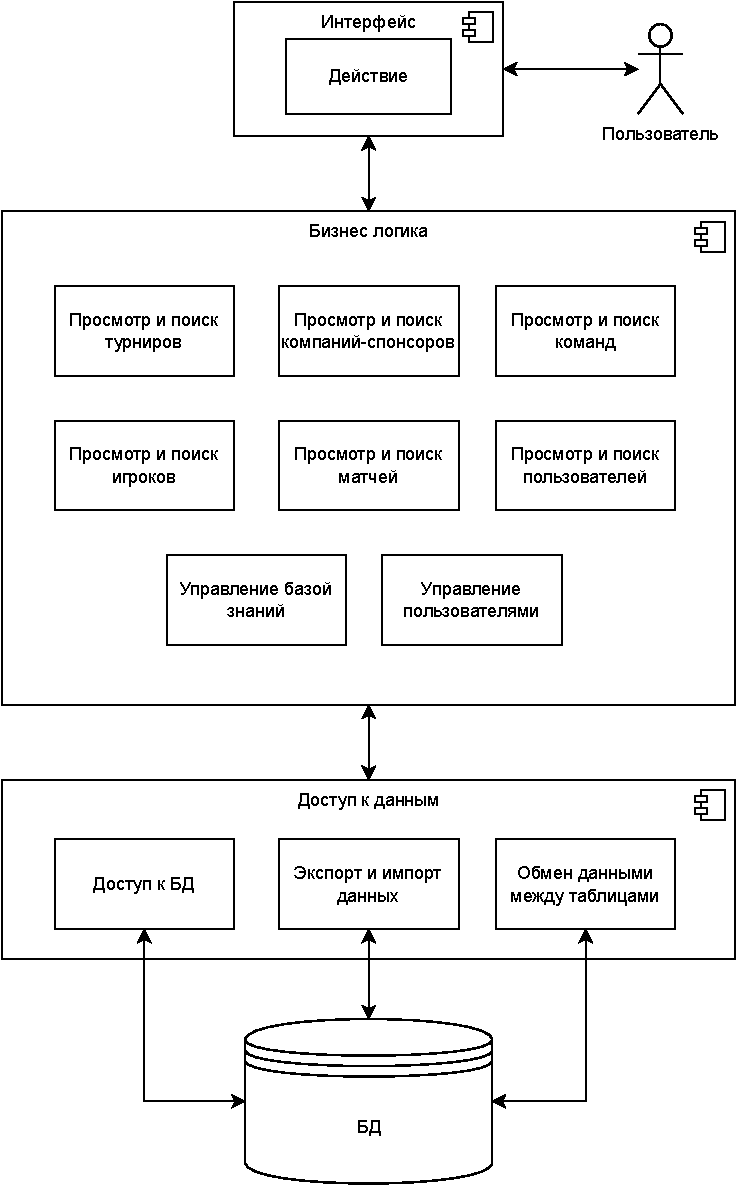
\includegraphics[scale = 0.9]{inc/diag/components.pdf}
	\caption{Высокоуровневое разбиение на компоненты}
	\label{fig:components}	
\end{figure}

\clearpage


\section{Описание интерфейса программного продукта}


При запуске приложения пользователю предоставляется возможность регистрации и создания собственного аккаунта в системе или выполнить вход под уже имеющимся (рисунок \ref{fig:login}).

\begin{figure}[h!btp]
	\centering
	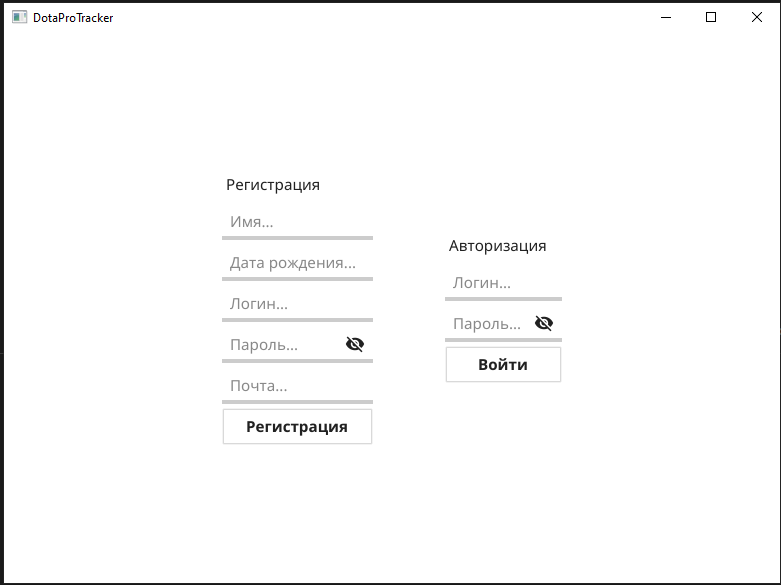
\includegraphics[scale = 0.7]{inc/img/login.png}
	\caption{Стартовое окно приложения}
	\label{fig:login}	
\end{figure}

После выполнения процедуры идентификации происходит процедура аутентификации пользователя (выполняется проверка соотвествия пароля введенного пользователем, с соответствующим паролем в базе данных, следует отметить, что пароли хранятся в зашифрованном виде с целью обеспечения сохранности и безопасности данных пользователей). В случае успешной аутентификации, пользователь получает доступ к функциям системы на основе своего уровня привилегий. На рисунке \ref{fig:admin} изображен интерфейс администратора.

\clearpage

\begin{figure}[h!btp]
	\centering
	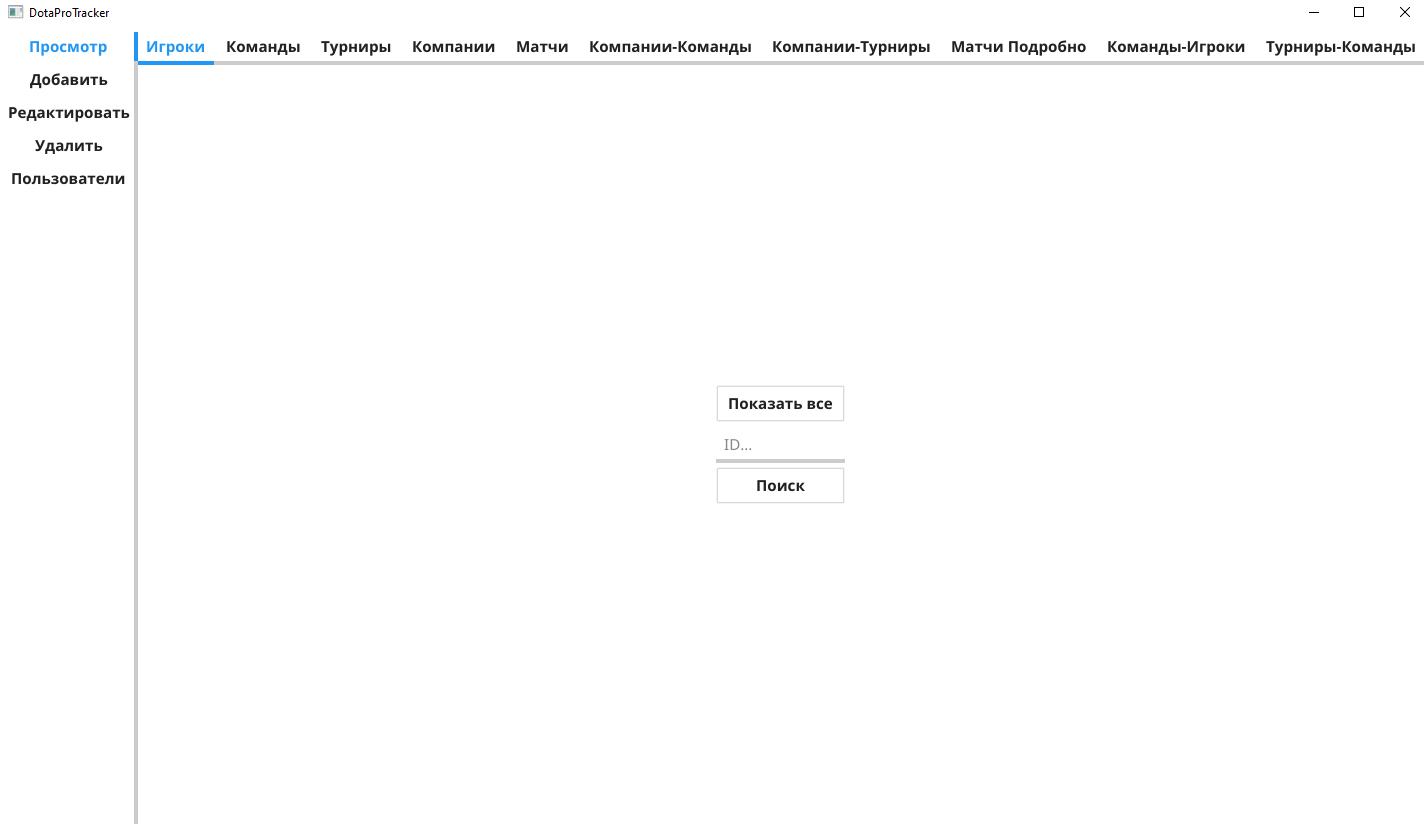
\includegraphics[scale = 0.4]{inc/img/admin.png}
	\caption{Интерфейс администратора}
	\label{fig:admin}	
\end{figure}

Администратор системы имеет право добавлять новых пользователей в систему, а также смотреть весь список существующих аккаунтов (рисунки \ref{fig:user_create}--\ref{fig:users}).


\begin{figure}[h!btp]
	\centering
	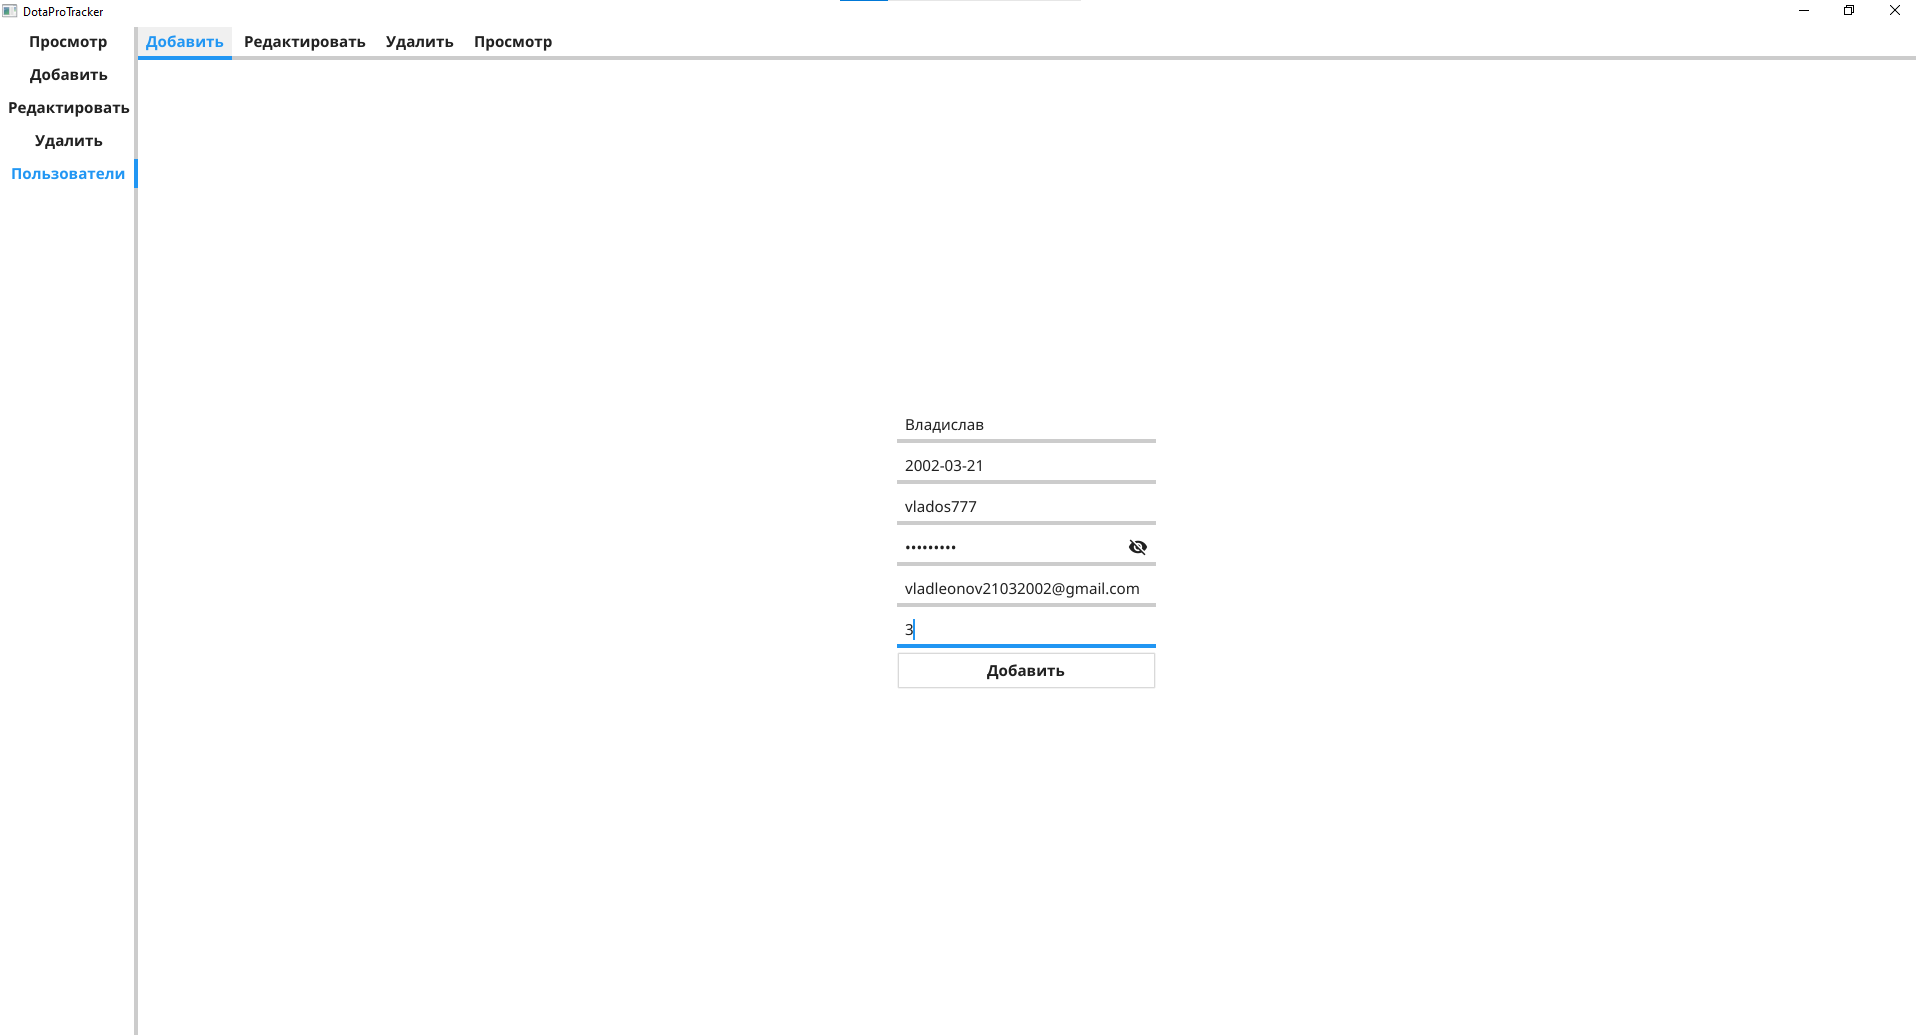
\includegraphics[scale = 0.3]{inc/img/user_create.png}
	\caption{Создание нового пользователя}
	\label{fig:user_create}	
\end{figure}


\clearpage

\begin{figure}[h!btp]
	\centering
	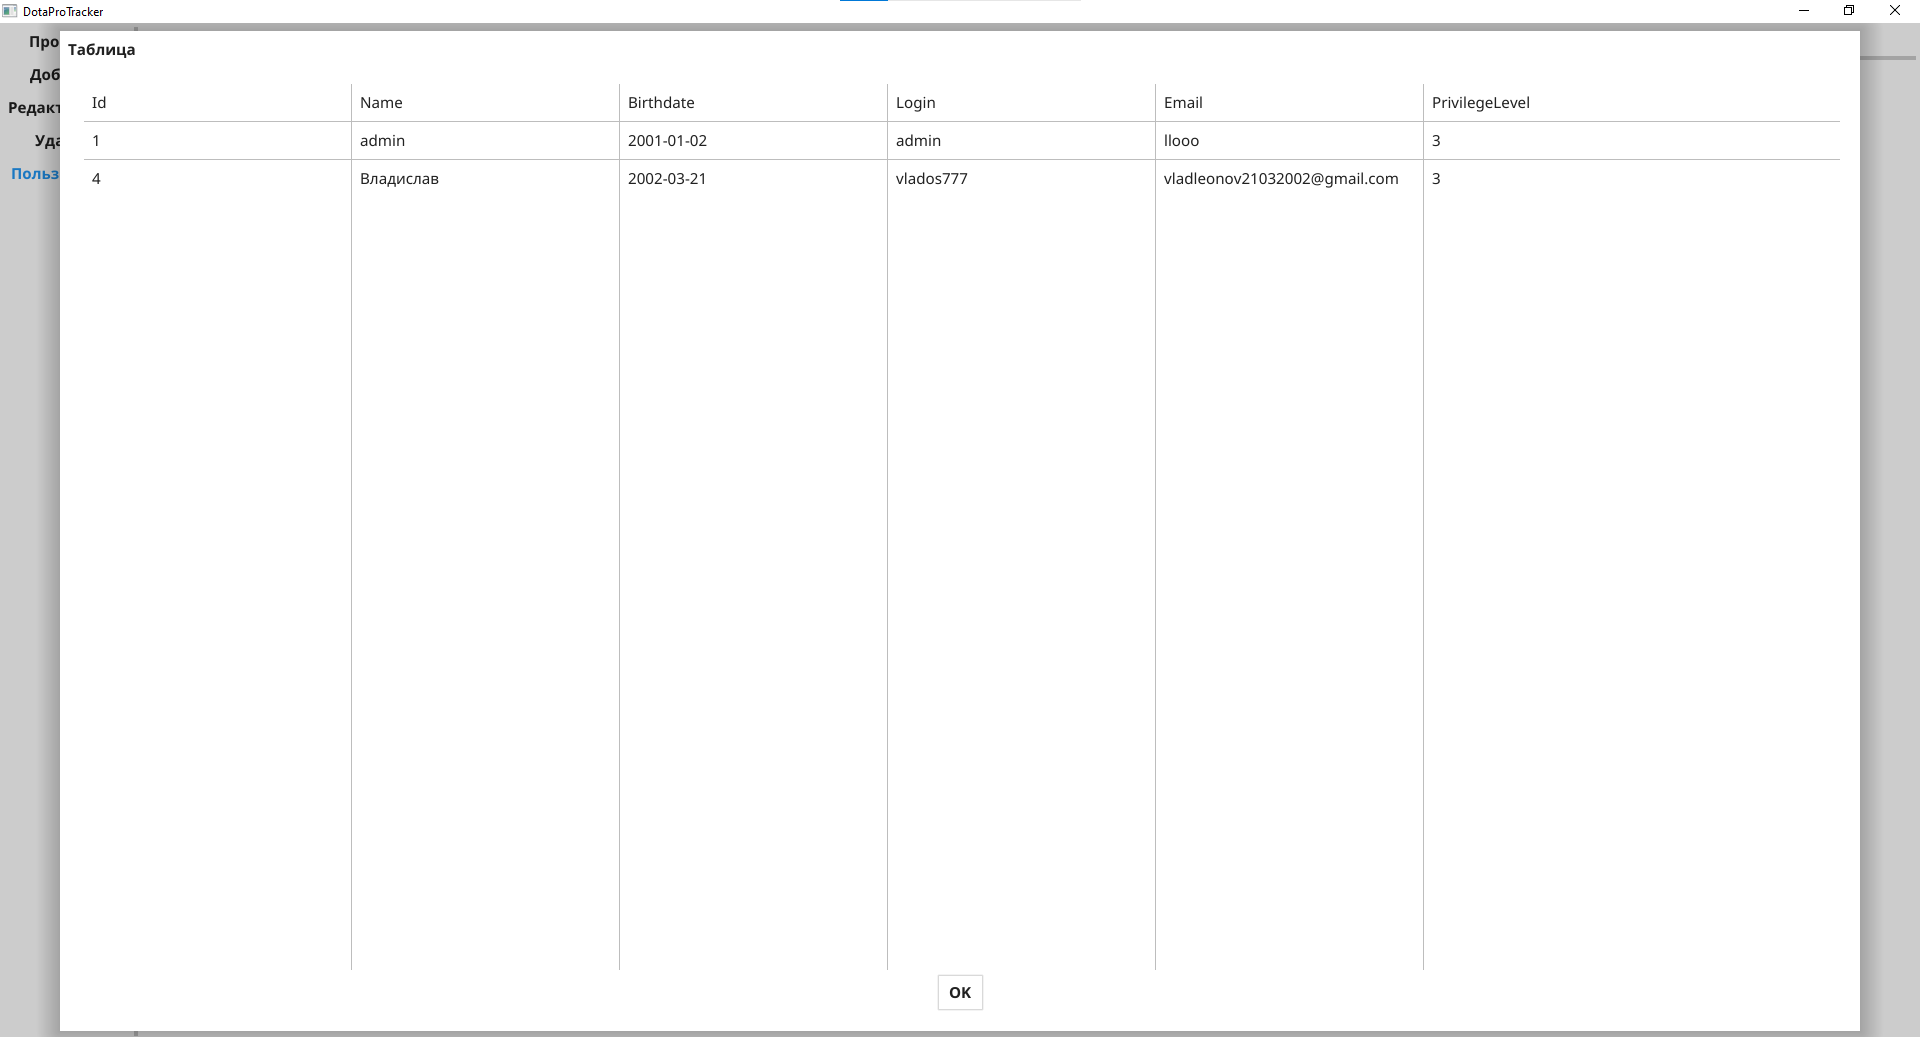
\includegraphics[scale = 0.3]{inc/img/users.png}
	\caption{Список существующих пользователей}
	\label{fig:users}	
\end{figure}

Роль модератора позволяет редактировать записи системы. Для навигации по записям реализована функция поиска (рисунки \ref{fig:edit}--\ref{fig:find})

\begin{figure}[h!btp]
	\centering
	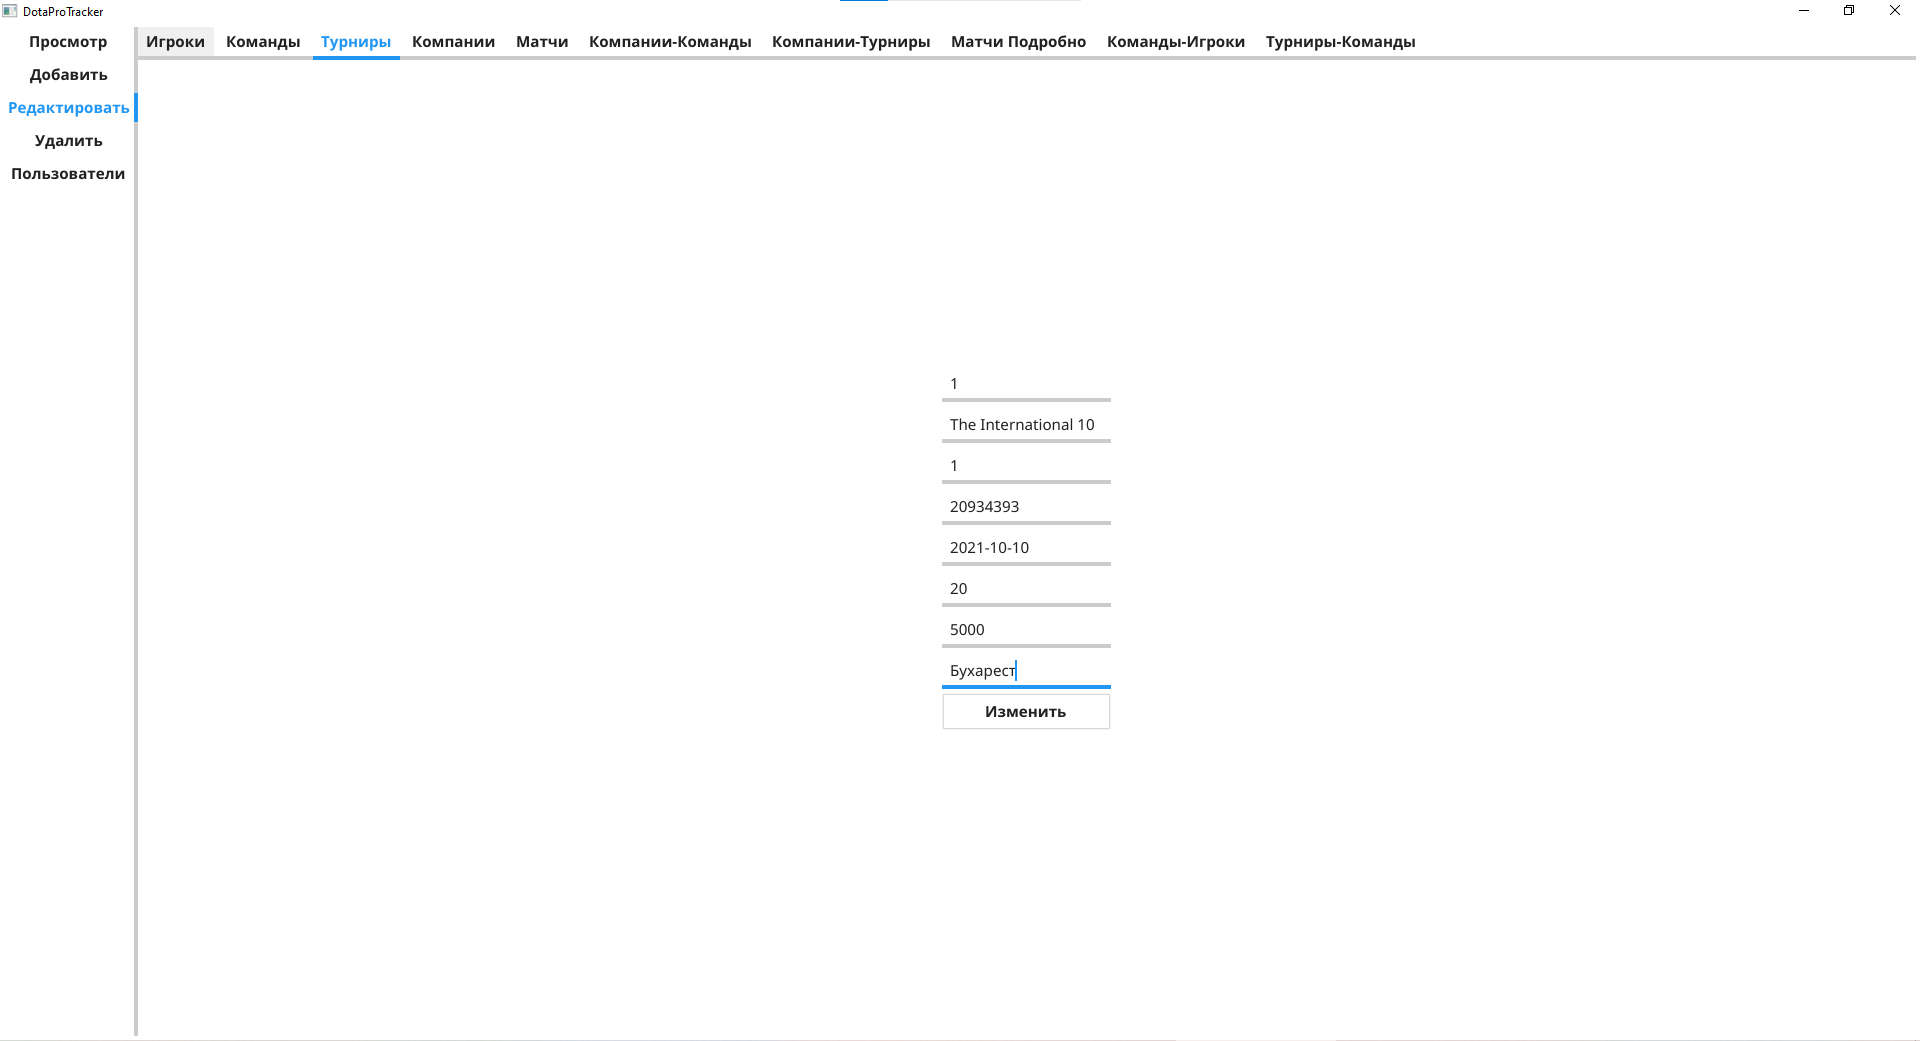
\includegraphics[scale = 0.3]{inc/img/edit.png}
	\caption{Редактирование записи о турнире}
	\label{fig:edit}	
\end{figure}

\clearpage

\begin{figure}[h!btp]
	\centering
	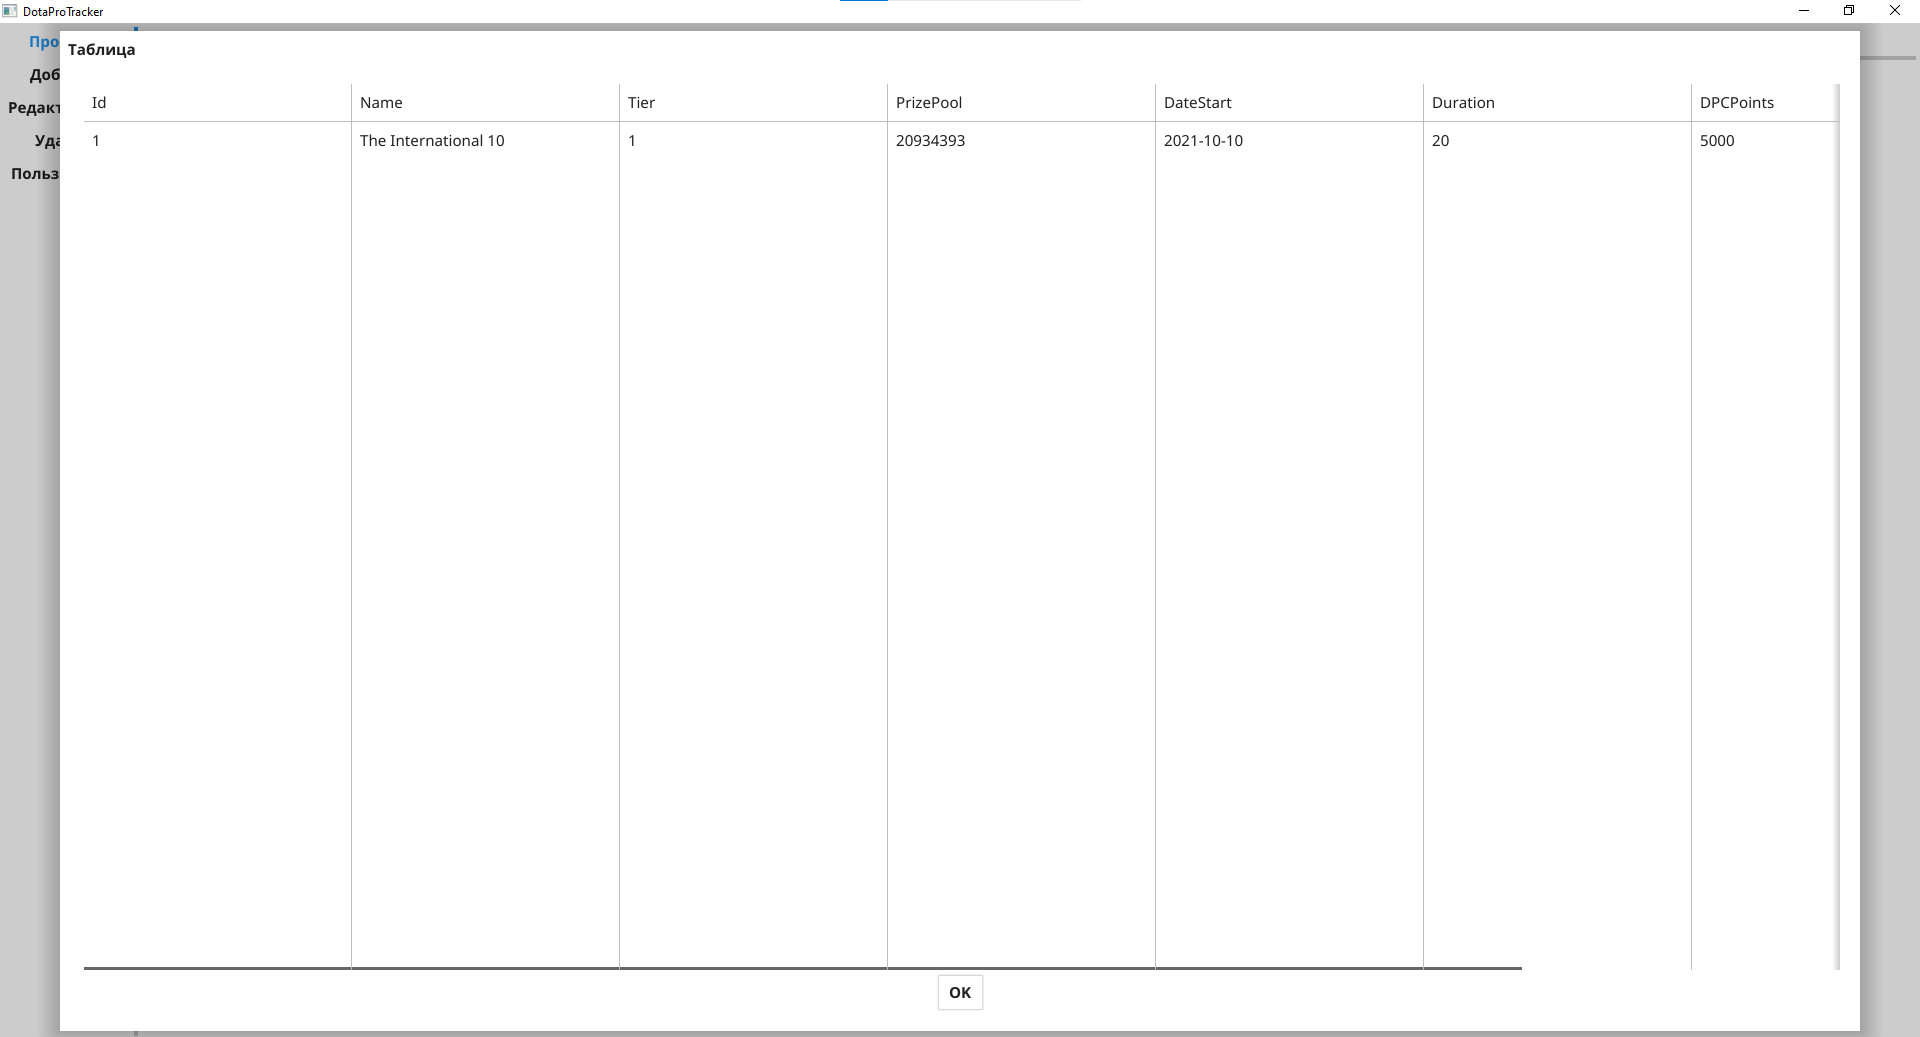
\includegraphics[scale = 0.3]{inc/img/find.png}
	\caption{Поиск записи о турнире}
	\label{fig:find}	
\end{figure}

Обычный пользователь имеет возможность просмотра и поиска записей (рисунок \ref{fig:companies}).

\begin{figure}[h!btp]
	\centering
	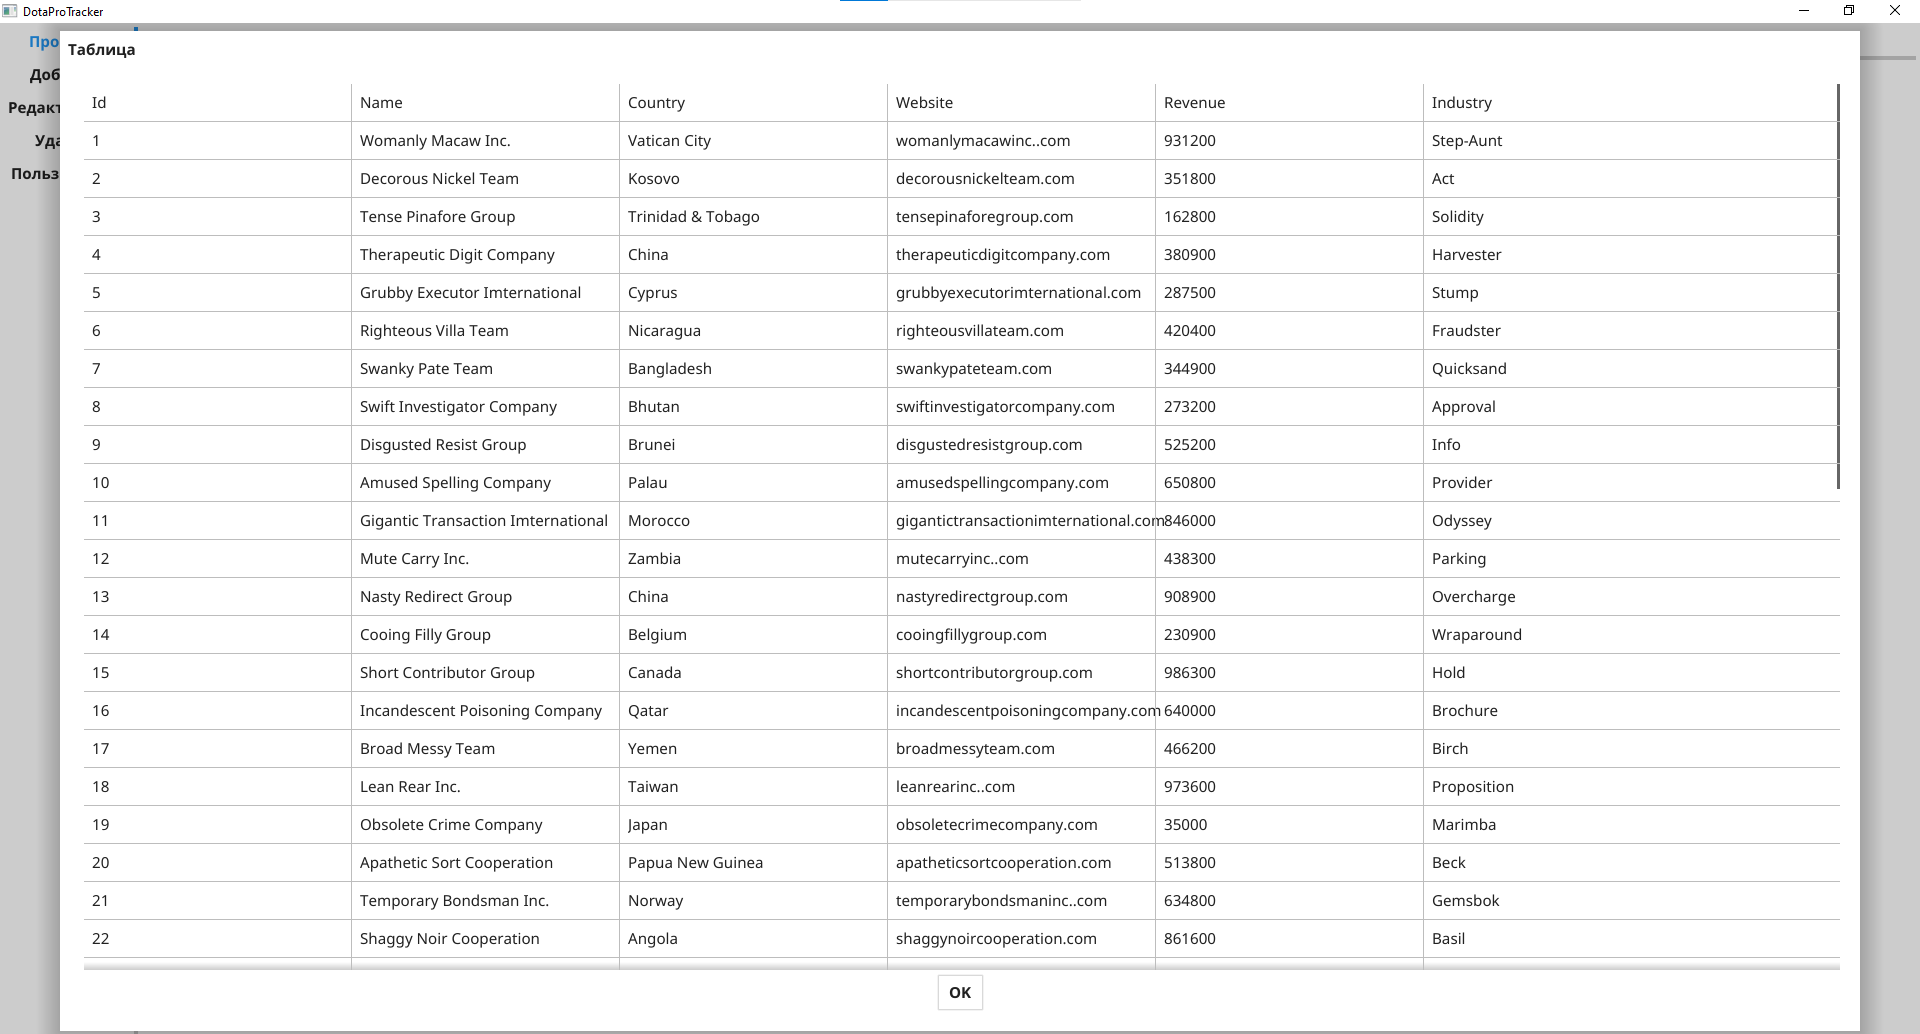
\includegraphics[scale = 0.3]{inc/img/companies.png}
	\caption{Просмотр записей о компаниях-спонсорах}
	\label{fig:companies}	
\end{figure}


\section*{Вывод}

В данном разделе были описаны выбранные технологии разработки, методология построения ПО, а также рассмотрено взаимодействие пользователя с приложением.''
\chapter{Исследовательский раздел}
\label{cha:research}

Технические характеристики устройства, на котором выполнялось тестирование:

\begin{itemize}
	\item Операционная система: Windows 10 64-bit \cite{windows}.
	\item Память: 16 GB.
	\item Процессор: AMD Ryzen 5 4600H \cite{amd} @ 3.00 GHz.
\end{itemize}

Тестирование проводилось на ноутбуке при включённом режиме производительности. Во время тестирования ноутбук был нагружен только системными процессами.

Предметом исследования является скорость выполнения запросов к базе данных в зависимости от использования/игнорирования процесса индексации записей в таблице методом бинарного дерева. Следует отметить, что запросы выполнялись на стороне базы данных в многократном количестве, после чего выполнялось усреднение полученных значений.

Индекс был создан по строковому полю \code{signature\_hero} таблицы \code{players}. В качестве тестового запроса был выбран следующий: 

\code{select * from players where signature\_hero = 'Riki';}

В результате эксперимента были полученные значения, представленные в таблице \ref{tabular:times}.


\begin{table}[h!]
	\centering
	\caption{\label{tabular:times}Сравнительный анализ времени выполнения запросов}
\begin{tabular}{|c|c|c|}
	\hline
	\textbf{Количество записей} & \textbf{С индексированием} & \textbf{Без индексирования} \\ \hline
	100 & 0.025 ms & 0.030 ms \\ \hline
	500 & 0.065 ms & 0.145 ms \\ \hline
	2000 & 0.080 ms & 0.475 ms \\ \hline
	5000 & 0.108 ms & 1.040 ms \\ \hline
	10000 & 0.176 ms & 1.976 ms \\ \hline
\end{tabular}
\end{table}

\section*{Вывод}

На основе полученных экспериментальным путем данных можно сделать вывод о том, что использование индексации позволяет существенным образом ускорить выполнение запроса (в ~11,22 раза для таблицы из 10000 записей). Однако следует учитывать тот факт, что на сравнительно небольших выборках данных индексация не дает столько значимого прироста быстродействия системы, а операция индексации требует дополнительной подготовки данных, а также увеличивает объем необходимой памяти для хранения. Так для исследуемой таблицы при 10000 записях потребовалось 88 Кбайт памяти для хранения дополнительных индексов (порядка 10\% от общей памяти, занимаемой таблицей).
\chapter*{ЗАКЛЮЧЕНИЕ}
\addcontentsline{toc}{chapter}{ЗАКЛЮЧЕНИЕ} 

В рамках курсовой работы была изучена предметная область для разрабатываемого программного продукта, рассмотрены существуюшие сервисы, выделены их основные характеристики и проведено сравнение, были описаны типы пользователей и возможные варианты взаимодействия с системой, проведена формализация данных и сущностей.

Цель курсовой работы была достигнута в полном объеме: была изучена предметная область, были выполнены проектирование и реализация базы данных, содержащей информацию о киберспортивных матчах и командах в дисциплине Dota 2, были созданы соответствующие триггеры и проведено исследование влияния индексации записей на скорость выполнения запросов в базе данных.

Следует отметить, что разработанное ПО в дальнейшем будет доработано посредством добавления системы анализа новых матчей на основе предыдущих, а также возможности просмотра прямых трансляций различных онлайн событий, проходящих в рамках конкретных турниров. 



\makebibliography

\begin{appendices}
\chapter{Создание базы данных}

Далее в листингах А.1--А.3 приведен сценарий создания базы данных.

\begin{lstlisting}[caption={Сценарий создания базы данных (часть 1)}]
	drop table if exists players cascade;
	drop table if exists teams cascade;
	drop table if exists tournaments cascade;
	drop table if exists companies cascade;
	drop table if exists teams_players cascade;
	drop table if exists companies_teams cascade;
	drop table if exists companies_tournaments cascade;
	drop table if exists tournaments_teams cascade;
	drop table if exists matches cascade;
	drop table if exists match_perfomances cascade;
	drop table if exists users cascade;
	
	create table "players" (
	"id" serial,
	"nickname" varchar,
	"realname" varchar,
	"birthdate" date,
	"country" varchar,
	"mmr" int,
	"role" varchar,
	"signature_hero" varchar
	);
	
	create table "teams" (
	"id" serial,
	"name" varchar,
	"created_at" date,
	"email" varchar,
	"total_earnings" int,
	"region" varchar,
	"tier" int
	);
\end{lstlisting}
\clearpage

\begin{lstlisting}[caption={Сценарий создания базы данных (часть 2)}]
	create table "tournaments" (
	"id" serial,
	"name" varchar,
	"tier" int,
	"prize_pool" int,
	"date_start" date,
	"duration" int,
	"dpc_points" int,
	"location" varchar
	);
	create table "companies" (
	"id" serial,
	"name" varchar,
	"country" varchar,
	"website" varchar,
	"revenue" int,
	"industry" varchar
	);
	create table "teams_players" (
	"id" serial,
	"team_id" int,
	"player_id" int,
	"contract_date" date,
	"contract_time" int
	);
	create table "companies_tournaments" (
	"id" serial,
	"company_id" int,
	"tournament_id" int,
	"deposit" int
	);
	create table "companies_teams" (
	"id" serial,
	"company_id" int,
	"team_id" int,
	"contract_date" date,
	"contract_time" int
	);
\end{lstlisting}
\clearpage

\begin{lstlisting}[caption={Сценарий создания базы данных (часть 3)}]
	create table "tournaments_teams" (
	"id" serial,
	"tournament_id" int,
	"team_id" int,
	"participation_type" varchar,
	"is_winner" boolean
	);
	create table "matches" (
	"id" serial,
	"tournament_id" int,
	"r_team_id" int,
	"d_team_id" int,
	"duration" int, 
	"winner" boolean
	);
	create table "users" (
	"id" serial,
	"name" varchar,
	"birthdate" date,
	"login" varchar, 
	"password" varchar,
	"email" varchar, 
	"privilege_level" int
	);
	create table "match_perfomances" (
	"id" serial,
	"match_id" int,
	"player_id" int, 
	"team" boolean,
	"hero" varchar,
	"kills" int,
	"deaths" int,
	"assists" int,
	"networth" int,
	"gpm" int,
	"xpm" int,
	"dmg" int,
	"heal" int,
	"bld" int
	);
\end{lstlisting}
\clearpage

\chapter{Ограничения в базе данных}

Далее в листингах Б.1--Б.4 приведен сценарий создания ограничений в базе данных. 

\begin{lstlisting}[caption={Сценарий создания ограничений в базе данных (часть 1)}]
	alter table "players" add constraint "players_id" primary key ("id"); 
	alter table "teams" add constraint "teams_id" primary key ("id");
	alter table "tournaments" add constraint "tournaments_id" primary key ("id");
	alter table "companies" add constraint "companies_id" primary key ("id");
	alter table "teams_players" add constraint "teams_players_id" primary key ("id");
	alter table "companies_tournaments" add constraint "companies_tournaments_id" primary key ("id");
	alter table "companies_teams" add constraint "companies_teams_id" primary key ("id");
	alter table "tournaments_teams" add constraint "tournaments_teams_id" primary key ("id");
	alter table "matches" add constraint "matches_id" primary key ("id");
	alter table "users" add constraint "users_id" primary key ("id");
	alter table "match_perfomances" add constraint "matches_perfomances_id" primary key ("id");
	alter table "teams_players" add foreign key ("team_id") references "teams" ("id") on delete cascade;
	alter table "teams_players" add foreign key ("player_id") references "players" ("id") on delete cascade;
	alter table "companies_tournaments" add foreign key ("company_id") references "companies" ("id") on delete cascade;
	alter table "companies_tournaments" add foreign key ("tournament_id") references "tournaments" ("id") on delete cascade;
	alter table "companies_teams" add foreign key ("company_id") references "companies" ("id") on delete cascade;
	alter table "companies_teams" add foreign key ("team_id") references "teams" ("id") on delete cascade;
	alter table "tournaments_teams" add foreign key ("tournament_id") references "tournaments" ("id") on delete cascade;
	alter table "tournaments_teams" add foreign key ("team_id") references "teams" ("id") on delete cascade;
	alter table "matches" add foreign key ("tournament_id") references "tournaments" ("id") on delete cascade;
	alter table "matches" add foreign key ("r_team_id") references "teams" ("id") on delete cascade;
	alter table "matches" add foreign key ("d_team_id") references "teams" ("id") on delete cascade;
\end{lstlisting}

\clearpage

\begin{lstlisting}[caption={Сценарий создания ограничений в базе данных (часть 2)}]
	alter table "match_perfomances" add foreign key ("match_id") references "matches" ("id") on delete cascade;
	alter table "match_perfomances" add foreign key ("player_id") references "players" ("id") on delete cascade;
	
	alter table "players" alter column "nickname" set not null;
	alter table "players" alter column "realname" set not null;
	alter table "players" alter column "birthdate" set not null;
	alter table "players" alter column "country" set not null;
	alter table "players" alter column "mmr" set not null;
	alter table "players" alter column "role" set not null;
	alter table "players" alter column "signature_hero" set not null;
	alter table "players" add constraint "players_mmr_check" check (mmr > 0);
	
	alter table "teams" alter column "name" set not null;
	alter table "teams" alter column "created_at" set not null;
	alter table "teams" alter column "email" set not null;
	alter table "teams" alter column "total_earnings" set not null;
	alter table "teams" alter column "region" set not null;
	alter table "teams" alter column "tier" set not null;
	alter table "teams" add constraint "teams_total_earnings_check" check (total_earnings > 0);
	alter table "teams" add constraint "teams_tier_check" check (tier > 0 and tier < 5);
	
	alter table "tournaments" alter column "name" set not null;
	alter table "tournaments" alter column "tier" set not null;
	alter table "tournaments" alter column "prize_pool" set not null;
	alter table "tournaments" alter column "date_start" set not null;
	alter table "tournaments" alter column "duration" set not null;
	alter table "tournaments" alter column "dpc_points" set not null;
	alter table "tournaments" alter column "location" set not null;
	alter table "tournaments" add constraint "tournaments_tier_check" check (tier > 0 and tier < 5);
	alter table "tournaments" add constraint "tournaments_prize_pool_check"check (prize_pool > 0);
	alter table "tournaments" add constraint "tournaments_date_check" check (duration > 0);
	alter table "tournaments" add constraint "tournaments_dpc_points_check"check (dpc_points >= 0);
\end{lstlisting}

\clearpage

\begin{lstlisting}[caption={Сценарий создания ограничений в базе данных (часть 3)}]	
	alter table "companies" alter column "name" set not null;
	alter table "companies" alter column "country" set not null;
	alter table "companies" alter column "website" set not null;
	alter table "companies" alter column "revenue" set not null;
	alter table "companies" alter column "industry" set not null;
	alter table "companies" add constraint "companies_revenue" check (revenue > 0);
	
	alter table "teams_players" alter column "team_id" set not null;
	alter table "teams_players" alter column "player_id" set not null;
	alter table "teams_players" alter column "contract_date" set not null;
	alter table "teams_players" alter column "contract_time" set not null;
	alter table "teams_players" add constraint "teams_players_contract_time_check" check (contract_time > 0 and contract_time <= 36);
	
	alter table "companies_tournaments" alter column "company_id" set not null;
	alter table "companies_tournaments" alter column "tournament_id" set not null;
	alter table "companies_tournaments" alter column "deposit" set not null;
	alter table "companies_tournaments" add constraint "companies_tournaments_deposit_check" check (deposit > 0);
	
	alter table "companies_teams" alter column "company_id" set not null;
	alter table "companies_teams" alter column "team_id" set not null;
	alter table "companies_teams" alter column "contract_date" set not null;
	alter table "companies_teams" alter column "contract_time" set not null;
	alter table "companies_teams" add constraint "companies_teams_contract_time_check" check (contract_time > 0 and contract_time <= 36);
	
	alter table "tournaments_teams" alter column "tournament_id" set not null;
	alter table "tournaments_teams" alter column "team_id" set not null;
	alter table "tournaments_teams" alter column "participation_type" set not null;
	alter table "tournaments_teams" alter column "is_winner" set not null;
	alter table "tournaments_teams" add constraint "tournaments_teams_participation_type_check" check (participation_type in ('invite', 'qualification'));
	
\end{lstlisting}

\clearpage

\begin{lstlisting}[caption={Сценарий создания ограничений в базе данных (часть 4)}]
	alter table "matches" alter column "tournament_id" set not null;
	alter table "matches" alter column "r_team_id" set not null;
	alter table "matches" alter column "d_team_id" set not null;
	alter table "matches" alter column "duration" set not null;
	alter table "matches" alter column "winner" set not null;
	alter table "matches" alter column "matches_duration_check" check (duration > 0);
	alter table "users" alter column "name" set not null;
	alter table "users" alter column "birthdate" set not null;
	alter table "users" alter column "login" set not null;
	alter table "users" alter column "password" set not null;
	alter table "users" alter column "email" set not null;
	alter table "users" alter column "privilege_level" set not null;
	alter table "users" add constraint "users_login" unique (login);
	alter table "users" add constraint "users_lvl_check" check (privilege_level > 0 and privilege_level < 4);
	alter table "match_perfomances" alter column "match_id" set not null;
	alter table "match_perfomances" alter column "player_id" set not null;
	alter table "match_perfomances" alter column "team" set not null;
	alter table "match_perfomances" alter column "hero" set not null;
	alter table "match_perfomances" alter column "kills" set not null;
	alter table "match_perfomances" alter column "deaths" set not null;
	alter table "match_perfomances" alter column "assists" set not null;
	alter table "match_perfomances" alter column "networth" set not null;
	alter table "match_perfomances" alter column "gpm" set not null;
	alter table "match_perfomances" alter column "xpm" set not null;
	alter table "match_perfomances" alter column "dmg" set not null;
	alter table "match_perfomances" alter column "heal" set not null;
	alter table "match_perfomances" alter column "bld" set not null;
	alter table "match_perfomances" add constraint "match_perfomances_kills_check" check (kills >= 0);
	alter table "match_perfomances" add constraint "match_perfomances_deaths_check" check (deaths >= 0);
	alter table "match_perfomances" add constraint "match_perfomances_assists_check" check (assists >= 0);
	alter table "match_perfomances" add constraint "match_perfomances_networth_check" check (networth > 0);
	alter table "match_perfomances" add constraint "match_perfomances_gpm_check" check (gpm > 0);
	alter table "match_perfomances" add constraint "match_perfomances_xpm_check" check (xpm > 0);
	alter table "match_perfomances" add constraint "match_perfomances_dmg_check" check (dmg >= 0);
	alter table "match_perfomances" add constraint "match_perfomances_heal_check" check (heal >= 0);
	alter table "match_perfomances" add constraint "match_perfomances_bld_check" check (bld >= 0);
\end{lstlisting}

\chapter{Ролевая модель}

Далее в листингах В.1--В.3 приведен сценарий создания ролевой модели в базе данных.

\begin{lstlisting}[caption={Сценарий создания ролевой модели в базе данных (часть 1)}]
	do
	$do$
	begin
	if exists (
	select from pg_catalog.pg_roles
	where  rolname = 'initial_login') then
	raise notice 'role "initial_login" already exists. skipping.';
	else
	create role initial_login with nosuperuser nocreatedb login password 'initial_login';
	end if;
	end
	$do$;
	do
	$do$
	begin
	if exists (
	select from pg_catalog.pg_roles
	where  rolname = 'default_user') then
	raise notice 'role "default_user" already exists. skipping.';
	else
	create role default_user with nosuperuser nocreatedb login password 'default_user';
	end if;
	end
	$do$;
	do
	$do$
	begin
	if exists (
	select from pg_catalog.pg_roles
	where  rolname = 'moderator') then
	raise notice 'role "moderator" already exists. skipping.';
	else
	create role moderator with nosuperuser nocreatedb login password 'moderator';
	end if;
	end
	$do$;
\end{lstlisting}

\clearpage

\begin{lstlisting}[caption={Сценарий создания ролевой модели в базе данных (часть 2)}]
	do
	$do$
	begin
	if exists (
	select from pg_catalog.pg_roles
	where  rolname = 'administrator') then
	raise notice 'role "administrator" already exists. skipping.';
	else
	create role administrator with nosuperuser nocreatedb login password 'administrator';
	end if;
	end
	$do$;
	
	grant select, insert on table users to initial_login;
	grant usage, select on sequence users_id_seq to initial_login;
	
	grant select on table players to default_user;
	grant select on table teams to default_user;
	grant select on table tournaments to default_user;
	grant select on table companies to default_user;
	grant select on table teams_players to default_user;
	grant select on table companies_teams to default_user;
	grant select on table companies_tournaments to default_user;
	grant select on table tournaments_teams to default_user;
	grant select on table matches to default_user;
	grant select on table match_perfomances to default_user;
	
	grant select, insert, delete, update on table players to moderator;
	grant select, insert, delete, update on table teams to moderator;
	grant select, insert, delete, update on table tournaments to moderator;
	grant select, insert, delete, update on table companies to moderator;
	grant select, insert, delete, update on table teams_players to moderator;
	grant select, insert, delete, update on table companies_teams to moderator;
	grant select, insert, delete, update on table companies_tournaments to moderator;
	grant select, insert, delete, update on table tournaments_teams to moderator;
	grant select, insert, delete, update on table matches to moderator;
	grant select, insert, delete, update on table match_perfomances to moderator;
\end{lstlisting}

\clearpage

\begin{lstlisting}[caption={Сценарий создания ролевой модели в базе данных (часть 3)}]
	grant usage, select on sequence players_id_seq to moderator;
	grant usage, select on sequence teams_id_seq to moderator;
	grant usage, select on sequence tournaments_id_seq to moderator;
	grant usage, select on sequence companies_id_seq to moderator;
	grant usage, select on sequence teams_players_id_seq to moderator;
	grant usage, select on sequence companies_teams_id_seq to moderator;
	grant usage, select on sequence companies_tournaments_id_seq to moderator;
	grant usage, select on sequence tournaments_teams_id_seq to moderator;
	grant usage, select on sequence matches_id_seq to moderator;
	grant usage, select on sequence match_perfomances_id_seq to moderator;
	
	grant select, insert, delete, update on table players to administrator;
	grant select, insert, delete, update on table teams to administrator;
	grant select, insert, delete, update on table tournaments to administrator;
	grant select, insert, delete, update on table companies to administrator;
	grant select, insert, delete, update on table teams_players to administrator;
	grant select, insert, delete, update on table companies_teams to administrator;
	grant select, insert, delete, update on table companies_tournaments to administrator;
	grant select, insert, delete, update on table tournaments_teams to administrator;
	grant select, insert, delete, update on table matches to administrator;
	grant select, insert, delete, update on table match_perfomances to administrator;
	grant select, insert, delete, update on table users to administrator;
	
	grant usage, select on sequence players_id_seq to administrator;
	grant usage, select on sequence teams_id_seq to administrator;
	grant usage, select on sequence tournaments_id_seq to administrator;
	grant usage, select on sequence companies_id_seq to administrator;
	grant usage, select on sequence teams_players_id_seq to administrator;
	grant usage, select on sequence companies_teams_id_seq to administrator;
	grant usage, select on sequence companies_tournaments_id_seq to administrator;
	grant usage, select on sequence tournaments_teams_id_seq to administrator;
	grant usage, select on sequence matches_id_seq to administrator;
	grant usage, select on sequence match_perfomances_id_seq to administrator;
	grant usage, select on sequence users_id_seq to administrator;
\end{lstlisting}

	\chapter{Триггеры}

Далее в листингах Г.1--Г.2 приведен сценарий создания триггеров в базе данных.

\begin{lstlisting}[caption={Сценарий создания триггеров в базе данных (часть 1)}]
	create or replace function make_deposit()
	returns trigger
	as
	$$
	begin
	update tournaments
	set prize_pool = prize_pool + new.deposit 
	where id = new.tournament_id;
	return new;
	end;
	$$ 
	language plpgsql;
	
	drop trigger if exists make_deposit_trigger on companies_tournaments;
	create trigger make_deposit_trigger after insert on companies_tournaments
	for row execute procedure make_deposit();
\end{lstlisting}

\clearpage

\begin{lstlisting}[caption={Сценарий создания триггеров в базе данных (часть 2)}]
	create or replace function make_win()
	returns trigger
	as
	$$
	declare
	tmp int = 0;
	begin
	if (new.is_winner = true) then 
	select into tmp prize_pool from tournaments_teams join tournaments
	on tournaments.id = tournaments_teams.id
	where tournaments.id = new.tournament_id;
	
	update teams
	set total_earnings = total_earnings + tmp
	where teams.id = new.team_id;
	end if;
	return new;
	end;
	$$ 
	language plpgsql;
	
	drop trigger if exists make_win on tournaments_teams;
	create trigger make_win after insert on tournaments_teams
	for row execute procedure make_win();
\end{lstlisting}

\clearpage


\end{appendices}

\end{document}